\documentclass[14pt]{article}
\usepackage{setspace}
\usepackage{enumitem}
\usepackage{graphicx}
\usepackage[table]{xcolor}
\usepackage[a4paper,margin=2cm]{geometry}
\usepackage{hyperref}
\usepackage{amsmath,amssymb,amsfonts}
\usepackage{booktabs}
\usepackage{float}
\usepackage{xepersian}

\settextfont{B Nazanin}
\setlatintextfont{TeX Gyre Termes}
\renewcommand{\labelitemi}{$\bullet$}

\usepackage[backend=biber,style=numeric,sorting=none,autolang=other]{biblatex}
\addbibresource{Report.bib}

\setstretch{1.15}
\graphicspath{{figs/}}

\usepackage{xspace}
\newcommand{\pt}{\ensuremath{p_\mathrm{T}}\xspace}
\newcommand{\bb}{\ensuremath{\mathrm{b}\bar{\mathrm{b}}}\xspace}
\newcommand{\Zbb}{\ensuremath{\mathrm{Z}\to\mathrm{b}\bar{\mathrm{b}}}\xspace}
\newcommand{\ttbb}{\ensuremath{\mathrm{t}\bar{\mathrm{t}}\mathrm{b}\bar{\mathrm{b}}}\xspace}
\newcommand{\bbbb}{\ensuremath{\mathrm{b}\bar{\mathrm{b}}\mathrm{b}\bar{\mathrm{b}}}\xspace}
\newcommand{\Zjet}{\ensuremath{\mathrm{Z{+}jet}}\xspace}
\newcommand{\ttZ}{\ensuremath{\mathrm{t}\bar{\mathrm{t}}\mathrm{Z}}\xspace}

\newcommand{\quadfig}[6]{%
\begin{figure}[H]\centering
\includegraphics[width=0.48\textwidth]{#1}\hfill\includegraphics[width=0.48\textwidth]{#2}\\[3pt]
\includegraphics[width=0.48\textwidth]{#3}\hfill\includegraphics[width=0.48\textwidth]{#4}
\caption{#5}\label{#6}
\end{figure}}
\newcommand{\widefig}[3]{%
\begin{figure}[H]\centering
\includegraphics[width=\textwidth]{#1}
\caption{#2}\label{#3}
\end{figure}}
\newcommand{\gridfig}[3]{%
\begin{figure}[H]\centering
\includegraphics[width=0.245\textwidth]{#1_pt}\hfill\includegraphics[width=0.245\textwidth]{#1_eta}\hfill\includegraphics[width=0.245\textwidth]{#1_mass}\hfill\includegraphics[width=0.245\textwidth]{#1_msd}\\[2pt]
\includegraphics[width=0.245\textwidth]{#1_girth}\hfill\includegraphics[width=0.245\textwidth]{#1_nconst}\hfill\includegraphics[width=0.245\textwidth]{#1_tau1}\hfill\includegraphics[width=0.245\textwidth]{#1_tau2}\\[2pt]
\includegraphics[width=0.245\textwidth]{#1_tau3}\hfill\includegraphics[width=0.245\textwidth]{#1_tau21}\hfill\includegraphics[width=0.245\textwidth]{#1_tau32}\hfill\includegraphics[width=0.245\textwidth]{#1_c2}\\[2pt]
\includegraphics[width=0.245\textwidth]{#1_d2}\hfill\includegraphics[width=0.245\textwidth]{#1_n2}\hfill\includegraphics[width=0.245\textwidth]{#1_zg}\hfill\includegraphics[width=0.245\textwidth]{#1_rg}
\caption{#2}\label{#3}
\end{figure}}
\newcommand{\Zbos}{\ensuremath{\mathrm{Z}}}
\newcommand{\bq}{\ensuremath{\mathrm{b}}}
\begin{document}

\begin{titlepage}
\thispagestyle{empty}

% Logos row
\noindent
\makebox[\paperwidth][l]{%
  \hspace*{-\oddsidemargin}%
  \hspace*{-1in}%
  
\includegraphics[width=4cm]{logo.png}%
  %\hfill
  \hspace*{3.25in}
  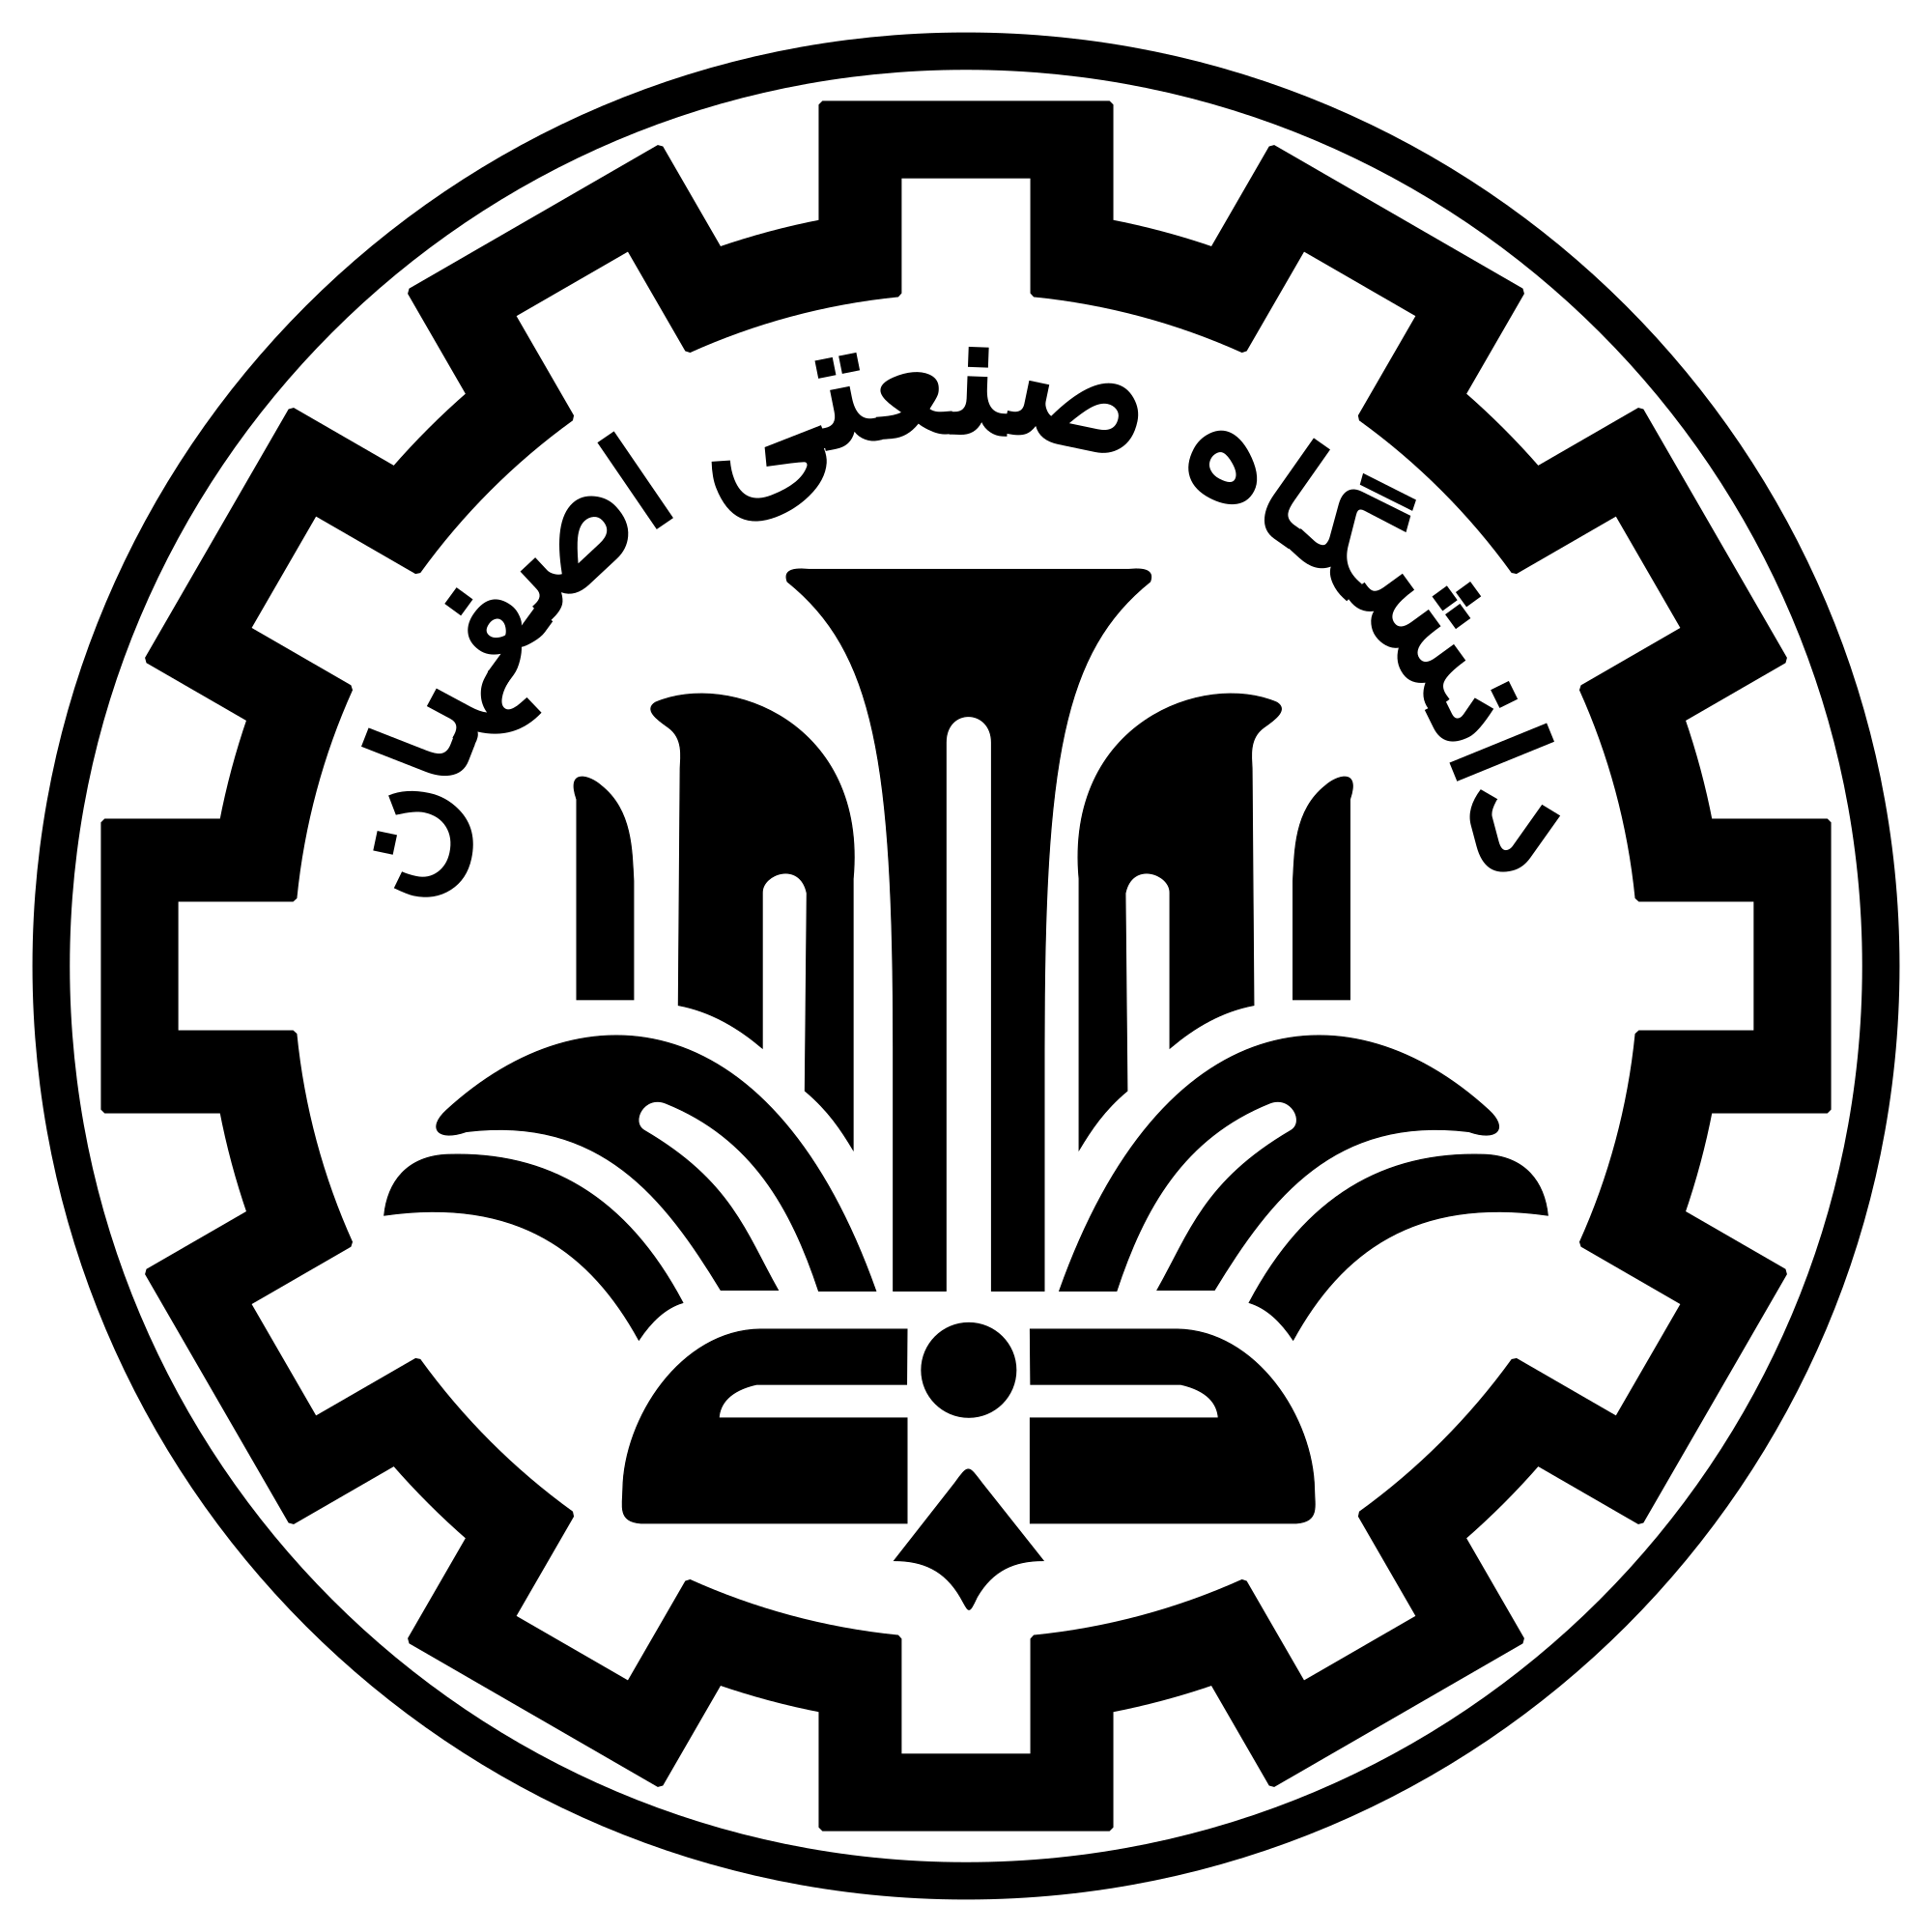
\includegraphics[width=3cm]{logoiut.png}%
}


\vspace{4cm}

\begin{center}
{\large\bfseries گزارش پیشرفت طرح}

\vspace{0.8cm}

{\LARGE\bfseries  یادگیری ماشین کوانتومی مضاعف}

\vspace{0.3cm}

{\LARGE\bfseries  برای کشف برهمکنش‌های نوین کوارک تاپ}

\vspace{0.7cm}

{\large\bfseries مرحله اول}

\vspace{4cm}

{\large\bfseries مجری طرح}

\vspace{0.3cm}

{\Large\bfseries عبیده جعفری}

\vspace{3cm}

{\large\bfseries آغاز: ۱ مرداد ۱۴۰۴}

%\vfill
\vspace{0.6cm}

{\large \bfseries  ارائه: \today }
\end{center}

\end{titlepage}


\newpage
\tableofcontents
\newpage

\section{مقدمه و هدف}
\label{sec:intro}
همان‌طور که در بخش قبلی گزارش دیدید، شناساگر (\lr{tagger}) جت‌های بوست‌شده \Zbb را طراحی کرده‌ایم. هدف این بخش تولید داده مناسب برای تشخیص رویدادهای \ttZ از پس‌زمینه \ttbb است؛ به این صورت که شناساگر جت‌های \lr{Z} را مشخص می‌کند و جداکننده رویداد (\lr{event discriminator}) با خروجی آن رویدادهای \ttZ را از \ttbb جدا می‌کند. برای اینکه تفاوت موجود در توزیع‌ها حاصل از روش تولید متفاوت نباشد و تنها ناشی از فیزیک فرایندها باشد، همه رویدادها را در یک چارچوب شبیه‌سازی واحد تولید کردیم: نسخه نرم‌افزارها، تعریف جت، برش‌های تحلیل، برچسب منشأ جت‌ها و قالب ذخیره‌سازی برای همه نمونه‌ها یکی است. از آنجا که شناساگر روی یک داده آموزش می‌بیند ولی خروجی آن را روی داده دوم، یعنی جت‌های رویدادهای \ttZ و \ttbb، می‌خواهیم، تمام تلاشمان این بود که پردازش دو داده یکسان باشد تا خروجی روی داده دوم تا حد ممکن منصفانه باشد. با این حال، این دو داده فرایندهای فیزیکی متفاوتی هستند، بنابراین توزیع‌های آنها همچنان کمی با هم فرق دارند.

برای ورودی شناساگر \lr{Z} یک نمونه سیگنال می‌سازیم که \lr{Z+jet} است: یک بوزون \lr{Z} پرتکانه همراه با یک جت تولید می‌شود و \lr{Z} به یک زوج \bb واپاشی می‌کند که در یک جت بوست‌شده جمع می‌شود. نمونه پس‌زمینه \lr{bbbb} است: چهار کوارک \lr{b} (دو زوج \bb) در برهمکنش \lr{QCD} تولید می‌شوند و جت بوست‌شده از یکی از این زوج‌ها ساخته می‌شود، یعنی جتی که \bb دارد ولی از \lr{Z} نیامده است. وقتی شناساگر \lr{Z} بین این دو نمونه تمایز ایجاد کند، خروجی آن به یک جداکننده کوانتومی داده می‌شود که سیگنال \ttZ را، یعنی تولید یک زوج کوارک تاپ همراه با بوزون \lr{Z} که به \bb وامی‌پاشد و علاوه بر جت \lr{Z} جت‌های ناشی از واپاشی تاپ‌ها را دارد، از پس‌زمینه \ttbb جدا کند؛ در \ttbb یک زوج تاپ همراه با یک زوج \bb از برهمکنش \lr{QCD} تولید می‌شود. از هر نمونه ۲۰۰۰۰ رویداد در برخورد \lr{pp} با انرژی \lr{13~TeV} ساخته شده است.

پرسش اصلی این است که آیا متغیرهای زیرساختار جت و ویژگی‌های ذره‌ها برای هر چهار نمونه رفتار هماهنگی دارند، و آیا شناساگری که روی یک جفت (سیگنال، پس‌زمینه) آموزش دیده روی جفت دیگر هم کار می‌کند.

در ادامه، بخش~\ref{sec:sim} زنجیره شبیه‌سازی، برش‌ها و برچسب منشأ جت‌ها را توضیح می‌دهد؛ بخش~\ref{sec:vars} متغیرهای جت و ذره را تعریف می‌کند. در بخش~\ref{sec:cutflow} تعداد جت‌ها بعد از هر برش آمده است و در بخش‌های~\ref{sec:set1} تا~\ref{sec:particles} نمودارهای چهار نمونه را کنار هم می‌گذاریم و مقایسه می‌کنیم. بخش~\ref{sec:disc} به بحث و محدودیت‌ها و بخش~\ref{sec:next} به گام بعدی اختصاص دارد.

\section{زنجیره شبیه‌سازی و نمونه‌ها}
\label{sec:sim}
ابتدا فرایند سخت را با \lr{MadGraph 3.5.3} در سطح پارتون تولید می‌کنیم. در این مرحله برش‌های زیر را اعمال می‌کنیم. این برش‌ها را طوری گذاشته‌ایم که جت‌های بوست‌شده‌ای تولید شود که هر دو کوارک \bq{} در آن جای بگیرند. وقتی \Zbos{} با تکانه عرضی بزرگ تولید می‌شود، زاویه بین دو محصول واپاشی کوچک می‌شود: تقریباً $\Delta R\approx 2m_\mathrm{Z}/\pt\approx 0.45$ برای \lr{$\pt=400$~GeV}. این مقدار از شعاع جت ($R=0.8$) کوچک‌تر است و هر دو \bq{} در یک جت می‌افتند. به همین دلیل در \lr{zj} و \ttZ روی \pt بوزون \Zbos{} برش \lr{$\pt(\mathrm{Z})>400$~GeV} گذاشته‌ایم. علاوه بر این برش‌ها، برش $|\eta|<2$ روی جت‌های بازسازی‌شده اعمال می‌شود.

پس‌زمینه‌ها هم باید در همان ناحیه بوست‌شده تولید شوند، وگرنه مقایسه با سیگنال منصفانه نیست و بیشتر رویدادها بعد از برش‌های تحلیل از بین می‌روند. در \ttbb برش روی \pt زوج \bb (بزرگ‌تر از ۴۰۰~\lr{GeV}) همین نقش را دارد، و شرط \lr{$\Delta R(\mathrm{b\bar{b}})<0.8$} دو کوارک \bq{} را به هم نزدیک می‌کند تا هر دو در یک جت با $R=0.8$ جای بگیرند و هندسه‌ای شبیه واپاشی \Zbos{} داشته باشیم.

همچنین برش‌های تحلیل، یعنی \lr{$\pt>400$~GeV} و \lr{$|\eta|<2$}، روی جت‌های بازسازی‌شده اعمال می‌شوند، چون پاسخ آشکارساز و تابش بیرون از مخروط جت دقیقاً یکی نیستند؛ بخشی از جت‌ها بعد از برش \pt زیر ۴۰۰ می‌افتند (جدول~\ref{tab:cutflow}).

سپس با \lr{MadSpin} ذرات سنگین را واپاشی می‌دهیم. در \lr{zj} و \ttZ بوزون \Zbos{} به یک زوج \bb واپاشی می‌کند. در \ttZ هر یک از دو کوارک تاپ به یک کوارک \bq{} و یک بوزون \lr{W} می‌پاشد و هر \lr{W} به یک لپتون باردار و نوترینوی متناظر آن؛ لپتون باردار الکترون یا میون است (در رویدادهای بررسی‌شده تقریباً نیمی الکترون و نیمی میون‌اند و لپتون تاو دیده نمی‌شود). در \ttbb هم دو تاپ دقیقاً به همین شکل، یعنی دولپتونی، واپاشی داده می‌شوند. \lr{MadSpin} همبستگی‌های اسپینی بین محصولات این واپاشی‌ها را حفظ می‌کند.

بعد از آن \lr{Pythia 8.312} بارش پارتونی و هادرونیزاسیون را انجام می‌دهد. در بارش پارتونی، کوارک‌ها و گلوئون‌های اولیه با تابش گلوئون و شکافت گلوئون به زوج کوارک، به تعداد زیادی پارتون با انرژی کمتر تبدیل می‌شوند. هادرونیزاسیون (\lr{hadronization}) مرحله بعد است: به دلیل محصورشدگی رنگ، کوارک‌ها و گلوئون‌ها نمی‌توانند به‌صورت آزاد وجود داشته باشند؛ در پایان بارش، آنها به هادرون‌های بی‌رنگ (مزون‌ها و باریون‌ها) تبدیل می‌شوند، که در \lr{Pythia} با مدل رشته لوند~\cite{Andersson:1983ia} انجام می‌شود. هادرون‌های ناپایدار سپس واپاشی می‌کنند تا ذرات پایانی بماند.

\lr{Delphes 3.5.1pre09} پاسخ آشکارساز را با تنظیمات موجود در آزمایش \lr{CMS} شبیه‌سازی می‌کند و خروجی آن ردهای باردار و اثرات آشکارشده در کالریمترها (فوتون و هادرون خنثی) است. در پایان \lr{FastJet 3.4.1} این ذره‌ها را به جت تبدیل می‌کند: جت‌ها با الگوریتم \lr{anti-$k_\mathrm{T}$} و $R=0.8$ ساخته می‌شوند، که ذره‌های سخت را اول با ذره‌های نرم اطرافشان ادغام می‌کند و جت‌های گرد و مخروطی می‌دهد؛ توضیح مرحله‌به‌مرحله آن در پیوست~\ref{app:antikt} آمده است. در \lr{FastJet} فقط جت‌هایی با \lr{$\pt>20$~GeV} ذخیره می‌شوند و بعد متغیرهای زیرساختار و ویژگی‌های ذره‌ها محاسبه و ذخیره می‌شوند.

برای هر کار خروجی هر مرحله (\lr{MadGraph}، \lr{MadSpin}، \lr{Pythia} و \lr{Delphes}) ذخیره شده و یک بذر تصادفی (\lr{random seed}) یکسان برای همه این مراحل به‌کار می‌رود. بذر هر کار از شناسه نمونه و شماره کار ساخته می‌شود و در یک پرونده ثبت می‌شود، پس کل زنجیره تکرارپذیر است و با همان بذر دقیقاً همان رویدادها دوباره به دست می‌آیند (\lr{FastJet} تصادفی نیست و به بذر نیازی ندارد). همه نمونه‌ها در مرتبه درختی (\lr{LO}) تولید شده‌اند و هر دو نمونه پس‌زمینه با فرایند \lr{QCD} خالص: \bbbb با \lr{QED=0}، یعنی دامنه بدون ثابت جفت‌شدگی الکتروضعیف، و \ttbb با \lr{WEIGHTED<=4}. \lr{WEIGHTED} مرتبه وزن‌دار ثابت‌های جفت‌شدگی در دامنه است که در \lr{MadGraph} هر توان $g_s$ را ۱ و هر توان $e$ را ۲ حساب می‌کند. دامنه $\mathrm{gg}\to t\bar t b\bar b$ فقط $g_s^4$ دارد، یعنی وزن ۴، و هر دیاگرام با $e$ وزن بیشتر از ۴ می‌شود و کنار می‌رود.

هنگام بازسازی جت‌ها، با توجه به مادر هر ذره‌ای که داخل جت قرار دارد، برای هر جت یک سری برچسب ثبت می‌کنیم که نشان می‌دهد جت از چه ذره‌هایی ساخته شده است، یعنی منشأ جت. جتی را که هر دو کوارک \bq{} حاصل از \Zbos{} داخل آن باشد جت کامل می‌نامیم و جتی را که فقط یکی از آن دو داخل آن باشد جت جزئی. در نهایت، در هر چهار فرایند این جت‌ها را بر اساس برچسب‌هایشان به سیگنال و پس‌زمینه تقسیم می‌کنیم: جت‌های کامل (و در حالتی دیگر جت‌های کامل و جزئی با هم) در دو نمونه سیگنال به‌عنوان سیگنال برداشته می‌شوند و جت‌هایی که \bq{} غیرتاپی دارند در دو نمونه پس‌زمینه به‌عنوان پس‌زمینه.

خلاصه‌ای از برش‌ها و برچسب‌های منشأ را در جدول~\ref{tab:samples} و جدول~\ref{tab:origin} می‌توانید ببینید.
\begin{table}[!ht]
\centering
\caption{نمونه‌ها و برش‌های سطح پارتون. در هر نمونه ۲۰ کار با ۱۰۰۰ رویداد، مجموعاً ۲۰۰۰۰ رویداد، اجرا شده است.}
\label{tab:samples}
\begin{tabular}{llp{6.5cm}}
\toprule
نمونه & نقش & برش سطح پارتون \\
\midrule
\lr{zj} & سیگنال & \lr{$\pt(\mathrm{Z})>400$~GeV}، بدون برش $\eta$ \\
\ttZ & سیگنال & \lr{$\pt(\mathrm{Z})>400$~GeV}، بدون برش $\eta$ \\
\bbbb & پس‌زمینه & چهار \bq{} به دو زوج با کمترین مجموع $\Delta R$ تقسیم می‌شوند و برای هر دو زوج \lr{$\pt>400$~GeV} و \lr{$\Delta R<0.8$} \\
\ttbb & پس‌زمینه & \lr{$\pt(\mathrm{b\bar{b}})>400$~GeV} و \lr{$\Delta R(\mathrm{b\bar{b}})<0.8$} \\
\bottomrule
\end{tabular}
\end{table}

\begin{table}[!ht]
\centering
\caption{برچسب‌های منشأ جت.}
\label{tab:origin}
\begin{tabular}{lp{10cm}}
\toprule
برچسب & معنی \\
\midrule
\lr{z\_both} & هر دو \bq{} حاصل از \Zbos{} داخل جت‌اند (جت کامل) \\
\lr{z\_part} & فقط یکی از دو \bq{} حاصل از \Zbos{} داخل جت است (جت جزئی) \\
\lr{nb\_notop} & تعداد \bq{}های داخل جت که از تاپ نیامده‌اند \\
\lr{nb\_top} & تعداد \bq{}های داخل جت که از تاپ آمده‌اند \\
\lr{n\_hard\_g}, \lr{n\_hard\_q} & تعداد گلوئون و کوارک سخت داخل جت \\
\lr{d\_z}, \lr{d\_top} & فاصله جت از \Zbos{} و از تاپ \\
\bottomrule
\end{tabular}
\end{table}

\section{ویژگی‌های جت‌ها و ذره‌ها}
\label{sec:vars}
برای هر جت یک مجموعه ویژگی زیرساختاری و سینماتیکی، و برای هر ذره داخل جت (تا ۱۰۰ ذره) ۱۷ ویژگی ذخیره می‌شود. در این بخش جزئیات این ویژگی‌ها را توضیح می‌دهیم.

\subsection{ویژگی‌های جت‌ها}
اولین ویژگی‌ها سینماتیکی‌اند. تکانه عرضی ($\pt$) مؤلفه تکانه عمود بر محور باریکه است، $\pt=\sqrt{p_x^2+p_y^2}$. شبه‌سرعت ($\eta$) از رابطه $\eta=-\ln\tan(\theta/2)$ به دست می‌آید که $\theta$ زاویه با محور باریکه است؛ مقدار صفر یعنی راستای عمود بر باریکه و مقدار بزرگ یعنی نزدیک به باریکه. زاویه سمتی ($\varphi$) زاویه در صفحه عمود بر باریکه است و فاصله زاویه‌ای ($\Delta R$) فاصله دو جسم در صفحه $(\eta,\varphi)$ را می‌دهد، $\Delta R=\sqrt{\Delta\eta^2+\Delta\varphi^2}$. جرم جت ($m$) جرم ناوردای مجموع چهارتکانه‌های همه ذرات تشکیل‌دهندهست، $m^2=\left(\sum_i p_i\right)^2$، و برای \Zbb قله‌ای نزدیک جرم \Zbos{} دارد.

پهنای جت ($g$) مجموع فاصله ذرات تشکیل‌دهنده از محور جت با وزن $\pt$ و نرمال‌شده با $\pt$ جت است، $g=\frac{1}{\pt^{\mathrm{jet}}}\sum_i \pt^{\,i}\,\Delta R_{i}$، و نشان می‌دهد انرژی جت چقدر از محور دور پخش شده است. ویژگی‌های مربوط به ساختار درونی جت ($\tau_1$، $\tau_2$، $\tau_3$) از رابطه $\tau_N=\frac{1}{d_0}\sum_i \pt^{\,i}\min\left(\Delta R_{i1},\dots,\Delta R_{iN}\right)$ با $d_0=R\sum_i\pt^{\,i}$ به دست می‌آیند که $\Delta R_{ik}$ فاصله ذره $i$ تا $k$-امین هسته جت است؛ مقدار کوچک $\tau_N$ یعنی جت با $N$ هسته سازگار است. نسبت‌های $\tau_{21}=\tau_2/\tau_1$ و $\tau_{32}=\tau_3/\tau_2$ وابستگی کمی به مقیاس کلی $\tau$ دارند: $\tau_{21}$ کوچک یعنی ساختار دو‌هسته‌ای (مانند \Zbb) و $\tau_{32}$ دو‌هسته‌ای را از سه‌هسته‌ای جدا می‌کند.

توابع همبستگی انرژی ($C_2$، $D_2$، $N_2$) بر پایه $e_2=\sum_{i<j} z_i z_j\,\Delta R_{ij}^{\beta}$ و $e_3=\sum_{i<j<k} z_i z_j z_k\,(\Delta R_{ij}\Delta R_{ik}\Delta R_{jk})^{\beta}$ ساخته می‌شوند که $z_i=\pt^{\,i}/\pt^{\mathrm{jet}}$ است؛ برای نمونه $C_2=e_3/e_2^2$ و $D_2=e_3/e_2^3$، و مانند $\tau_{21}$ ساختار دو‌هسته‌ای را می‌سنجند. در پایان، چند ویژگی از حذف ذره‌های نرم (\lr{soft-drop}) می‌آید که در آن ذره‌های نرمِ دور از هسته جت، یعنی آنهایی که سهم تکانه‌شان از جت کمتر از آستانه است، حذف می‌شوند. جرم پس از \lr{soft-drop} ($m_\mathrm{sd}$) جرم جت پس از این حذف است. سهم تکانه زیرجت نرم‌تر ($z_g$) برابر $z_g=\min(\pt^{(1)},\pt^{(2)})/(\pt^{(1)}+\pt^{(2)})$ برای دو زیرجت باقی‌مانده است و فاصله دو زیرجت ($R_g$) فاصله زاویه‌ای $\Delta R$ بین همان دو زیرجت است.

\subsection{ویژگی‌های ذره‌ها}
برای هر ذره داخل جت ۱۷ ویژگی ذخیره می‌شود که در آنها $\eta_\mathrm{jet}$ و $\varphi_\mathrm{jet}$ محور جت‌اند. مؤلفه‌های تکانه ($p_x$، $p_y$، $p_z$) و انرژی ($E$) ذره مستقیماً ذخیره می‌شوند و انرژی نسبی ($E_\mathrm{rel}$) برابر $E/E_\mathrm{jet}$ است. تکانه عرضی ($\pt$) و تکانه عرضی نسبی ($\pt^\mathrm{rel}=\pt/\pt^\mathrm{jet}$) نیز ذخیره می‌شوند. شبه‌سرعت ($\eta$) همراه با شبه‌سرعت نسبی ($\eta_\mathrm{rel}=\eta-\eta_\mathrm{jet}$) و زاویه سمتی ($\varphi$) همراه با زاویه سمتی نسبی ($\varphi_\mathrm{rel}=\varphi-\varphi_\mathrm{jet}$) ذخیره می‌شوند، که نسبی یعنی نسبت به محور جت. شبه‌سرعت چرخیده ($\eta_\mathrm{rot}$) و زاویه سمتی چرخیده ($\varphi_\mathrm{rot}$) به محور جت وابسته نیستند و در قابی تعریف می‌شوند که در ادامه شرح داده شده است. فاصله از محور جت ($\Delta R=\sqrt{\eta_\mathrm{rel}^2+\varphi_\mathrm{rel}^2}$)، کسینوس زاویه قطبی ذره ($\cos\theta=p_z/|\vec p|$، زاویه نسبت به محور باریکه) و کسینوس زاویه بین ذره و تکانه جت ($\cos\theta_\mathrm{rel}$) سه ویژگی دیگرند. آخرین ویژگی نوع ذره (\lr{pdgid}) است؛ برای ردهای باردار همان کد ذره در \lr{Delphes} است و برای اثرات آشکارشده در کالریمترها ۲۲ فوتون و ۱۳۰ هادرون خنثی را نشان می‌دهد. کدهای دیده‌شده ۱۱ (الکترون)، ۱۳ (میون)، ۲۲، ۱۳۰، ۲۱۱ (پیون باردار)، ۳۲۱ (کائون) و ۲۲۱۲ (پروتون) هستند.

برای ساختن قاب چرخیده، ابتدا مبدأ صفحه $(\eta,\varphi)$ را روی سخت‌ترین ذره جت می‌گذاریم، یعنی $\eta$ و $\varphi$ این ذره را از همه ذره‌ها کم می‌کنیم ($\varphi$ با در نظر گرفتن دوره‌ای بودن). سپس کل صفحه را آن‌قدر می‌چرخانیم که دومین ذره سخت روی محور منفی $\varphi$ بیفتد؛ زاویه چرخش از جهت همین ذره نسبت به محور $\eta$ به دست می‌آید. $\eta_\mathrm{rot}$ و $\varphi_\mathrm{rot}$ مؤلفه‌های هر ذره پس از این انتقال و چرخش‌اند. به همین دلیل $\eta_\mathrm{rot}$ و $\varphi_\mathrm{rot}$ ذره اول همیشه صفرند و ذره دوم فقط یک مؤلفه ناصفر دارد ($\varphi_\mathrm{rot}$ منفی)؛ از ذره سوم به بعد توزیع‌ها شکل ساختار دو‌هسته‌ای را نشان می‌دهند.

علاوه بر ویژگی‌ها، برای هر جت یک تصویر ۳۲$\times$۳۲ با وزن $\pt$ در صفحه $(\eta_\mathrm{rel},\varphi_\mathrm{rel})$ و بازه $\pm0.8$ ذخیره می‌شود. همه این‌ها در چهار فایل \lr{HDF5} با نام‌های \lr{events}، \lr{jet\_features}، \lr{constituents} و \lr{images} نگه داشته می‌شوند و پیوند رویداد$\to$جت$\to$ذره در آنها حفظ شده است.

\section{بررسی اثر برش‌ها}
\label{sec:cutflow}
جدول~\ref{tab:cutflow} تعداد جت‌های باقی‌مانده را بعد از هر برش نشان می‌دهد. ترتیب برش‌ها این است: ابتدا \lr{$\pt>20$~GeV} (آستانه ذخیره‌سازی)، سپس \lr{$|\eta|<2$}، سپس \lr{$\pt>400$~GeV} و در پایان انتخاب منشأ (فقط جت کامل).
\begin{table}[!ht]
\centering
\caption{تعداد جت‌ها بعد از هر برش (سیگنال: \lr{zj}، \ttZ؛ پس‌زمینه: \bbbb، \ttbb).}
\label{tab:cutflow}
\begin{tabular}{lrrrr}
\toprule
برش & \lr{zj} & \ttZ & \bbbb & \ttbb \\
\midrule
\lr{$\pt>20$~GeV} & 74083 & 110926 & 90296 & 120574 \\
\lr{+ $|\eta|<2$} & 59905 & 90106 & 70128 & 96717 \\
\lr{+ $\pt>400$~GeV} & 28450 & 20871 & 24653 & 18500 \\
\lr{+ full} & 11733 & 14056 & 23071 & 12532 \\
\lr{full + partial} & 13197 & 14934 & 24375 & 13648 \\
\bottomrule
\end{tabular}
\end{table}

\widefig{origin_counts.pdf}{تعداد جت‌ها به تفکیک منشأ در هر نمونه، بدون برش، فقط با برش $|\eta|<2$، فقط با برش $\pt>400$ و با هر دو برش (محور عمودی لگاریتمی).}{fig:origcounts}
\widefig{origin_fractions.pdf}{سهم هر منشأ از کل جت‌های هر نمونه در همان چهار حالت.}{fig:origfrac}
شکل‌های~\ref{fig:origcounts} و~\ref{fig:origfrac} نشان می‌دهند هر برش چه سهمی از جت‌ها را حذف می‌کند و جت‌های باقی‌مانده از چه منشأیی‌اند. برش $\pt>400$ مؤثرترین برش است: تعداد جت‌ها را چند برابر کم می‌کند و بیشتر جت‌های نرم با منشأ پرتوهای اولیه، رویداد زمینه و تابش نرم را حذف می‌کند، در حالی که برش $|\eta|<2$ اثر کمتری دارد. در نتیجه سهم جت‌های دارای زوج \bb از تاپ‌نیامده در \bbbb از حدود ۴۲ درصد به حدود ۹۴ درصد و در \ttbb از حدود ۱۶ درصد به حدود ۶۸ درصد می‌رسد، و سهم جت‌های \Zbos{}$\to$\bb در \ttZ از حدود ۱۷ درصد به حدود ۶۷ درصد و در \lr{zj} از حدود ۲۳ درصد به حدود ۴۱ درصد. بخش بزرگ باقی‌مانده در \lr{zj} کوارک سبک سخت (حدود ۴۳ درصد) و در \ttZ و \ttbb جت‌هایی‌اند که \bq{} آنها از تاپ می‌آید (حدود ۲۳ درصد).

\label{sec:set1}
در این بخش توزیع هفت متغیر جت را برای هر چهار نمونه با هم نشان می‌دهیم: \pt، $\eta$، جرم، \lr{girth}، تعداد مؤلفه‌ها (\lr{nconst})، فاصله $\Delta R$ تا نزدیک‌ترین جت دیگر و تعداد جت در رویداد. هر متغیر در چهار مرحله برش رسم شده است تا ببینیم هر برش شکل توزیع‌ها را چطور تغییر می‌دهد. همه توزیع‌ها به مساحت واحد نرمال شده‌اند، مگر نمودارهای تعداد جت در رویداد که کسر رویدادها را نشان می‌دهند.

در هر یک از شکل‌های این مجموعه، چهار نمودار چهار مرحله برش را نشان می‌دهند: \lr{$\pt>20$}، \lr{+$|\eta|<2$}، \lr{+$\pt>400$}، و آخر داده نهایی.

\quadfig{s1_pT20_pt.pdf}{s1_eta_pt.pdf}{s1_pt400_pt.pdf}{s1_sel_pt.pdf}{توزیع \pt جت بعد از هر برش.}{fig:s1pt}
در مرحله اول (\lr{$\pt>20$}) توزیع \pt دو بخش دارد: یک بخش با افت تقریباً نمایی در \pt کم و یک برجستگی نزدیک ۴۰۰ تا ۵۰۰~\lr{GeV}. این برجستگی همان جت بوست‌شده‌ای است که برش پارتونی \lr{$\pt>400$} تولید می‌کند. بعد از برش \lr{$\pt>400$} فقط همین جت‌ها می‌مانند و توزیع یکنواخت می‌شود و تقریباً نمایی می‌افتد.

دو نکته درباره توزیع \pt جت‌ها لازم به ذکر است. نخست اینکه در \pt بالای ۷۰۰~\lr{GeV} جت‌های \ttZ و \ttbb نسبت به \Zjet و \bbbb کمی بیشترند، یعنی دم توزیع در دو فرایند حاوی تاپ سخت‌تر است. دوم اینکه افزایش ظاهری در آخرین \lr{bin} اثر نمایشی است، چون جت‌های بالای ۱۵۰۰~\lr{GeV} در آخرین \lr{bin} جمع می‌شوند.

دم سخت‌تر در فرایندهای حاوی تاپ می‌تواند چند دلیل داشته باشد که با نمودارهای این گزارش جور درمی‌آید. نخست، تفاوت از خود \Zbos{} شروع می‌شود: در خروجی \lr{MadGraph} سهم \Zbos{}هایی با $\pt>700$~\lr{GeV} در \ttZ حدود \lr{6.7} درصد و در \Zjet حدود \lr{5.6} درصد است (شکل~\ref{fig:lhe-prod})، با اینکه برش مولد در هر دو یکسان است ($\pt(\mathrm{Z})>400$~\lr{GeV}). این می‌تواند از انرژی بزرگ‌تر فرایند سخت در فرایندهای حاوی تاپ بیاید، چون میانه $\sqrt{\hat s}$ در \ttZ برابر ۱۴۹۲~\lr{GeV} در برابر ۱۰۴۸ در \Zjet و در \ttbb برابر ۱۵۱۲ در برابر ۱۱۰۶ در \bbbb است (بخش~\ref{sec:zorigin})، و انرژی بیشتر تکانه بیشتری برای \Zbos{} و سیستم همراهش باقی می‌گذارد. دوم، آلودگی ناشی از واپاشی تاپ است: در \ttZ حدود \lr{8.3} درصد از جت‌های کامل \Zbos{} دست‌کم یک \bq{} از تاپ دارند و تکانه این ذره‌های اضافه به جت افزوده می‌شود، در حالی که در \Zjet چنین منبعی وجود ندارد. سوم، قطبش \Zbos{} است: کسر طولی در \ttZ برابر $f_L\approx0.57$ و در \Zjet برابر \lr{0.07} است، و \Zbos{} طولی تکانه را متقارن‌تر بین دو \bq{} پخش می‌کند و آنها را به هم نزدیک‌تر می‌کند، پس \Zbos{} بهتر در مخروط $R=0.8$ جا می‌گیرد و تکانه کمتری بیرون از جت می‌ماند. نشانه این اثر سهم جت‌های جزئی است که در \Zjet حدود ۱۱ درصد و در \ttZ حدود ۶ درصد است؛ این جت‌ها \Zbos{} را در مخروط دارند ولی کمتر از دو \bq{} و در نتیجه بخشی از تکانه \Zbos{} را از دست داده‌اند.

برای \ttbb در برابر \bbbb باید به برش‌های مولد هم توجه کرد، چون با هم فرق دارند: در \bbbb هر دو زوج باید $\pt>400$~\lr{GeV} و $\Delta R<0.8$ داشته باشند، ولی در \ttbb فقط یک زوج با $\pt>400$~\lr{GeV} و $\Delta R<0.8$. ساختار پس‌زدن هم فرق دارد: بعد از برش‌های $|\eta|<2$ و $\pt>400$ حدود ۵۱ درصد رویدادهای \Zjet و ۴۰ درصد \bbbb دو جت دارند و جت دیگر پشت‌به‌پشت جت منتخب است (قله $\Delta R\approx\pi$ در شکل~\ref{fig:s1dr})، ولی در \ttZ و \ttbb این سهم فقط حدود ۲۲ و ۱۸ درصد است (شکل~\ref{fig:s1njets}).

\quadfig{s1_pT20_eta.pdf}{s1_eta_eta.pdf}{s1_pt400_eta.pdf}{s1_sel_eta.pdf}{توزیع $\eta$ جت بعد از هر برش.}{fig:s1eta}
بدون برش \lr{$\eta$}، توزیع‌ها تا $|\eta|\approx5$ ادامه دارند و برای چهار نمونه تقریباً یکسان‌اند. بعد از برش \lr{$\pt>400$} جت‌ها مرکزی‌تر می‌شوند. در شکل نهایی \ttZ مرکزی‌ترین نمونه است (قله بلندتر در $\eta=0$)، \Zjet تخت‌ترین، و \bbbb و \ttbb بین آنها قرار دارند. این تفاوت در خود \Zbos{} هم هست و علتش آستانه انرژی فرایند سخت است. اگر دو پارتون ورودی کسرهای $x_1$ و $x_2$ از تکانه پروتون را داشته باشند، انرژی مرکز جرم فرایند سخت $\hat s=x_1x_2S$ و تندی سیستم $y=\frac12\ln(x_1/x_2)$ است، که $S=(13~\mathrm{TeV})^2$ مربع انرژی مرکز جرم برخورد دو پروتون است. از این دو رابطه $x_{1,2}=\sqrt{\hat s/S}\,e^{\pm y}$ به دست می‌آید و چون $x_{1,2}\le1$ است، همیشه $|y|\le\ln(\sqrt{S}/\sqrt{\hat s})$ است. پس هر چه $\sqrt{\hat s}$ بزرگ‌تر باشد بازه مجاز $y$ باریک‌تر می‌شود و رویدادها به مرکز نزدیک‌تر می‌شوند. \Zbos{} و جت مقابلش در جهت عرضی تعادل دارند و $\eta$ جت تندی همین سیستم را دنبال می‌کند: برای ذره‌ای که جرمش در برابر تکانه‌اش ناچیز است، یعنی سرعتش به سرعت نور نزدیک است، تندی $y$ تقریباً با شبه‌سرعت $\eta$ برابر است، و جت‌های ما با $\pt>400$~\lr{GeV} در همین وضعیت‌اند. پس سیستم باریک‌تر یعنی جت مرکزی‌تر. در \ttZ علاوه بر \Zbos{} باید دو تاپ هم ساخته شوند، پس کمینه $\sqrt{\hat s}$ بالاتر است: با $\pt(\mathrm{Z})>400$~\lr{GeV} این کمینه تقریباً ۸۱۰~\lr{GeV} برای \Zjet و ۹۴۰~\lr{GeV} برای \ttZ است. داده همین را نشان می‌دهد: میانه $\sqrt{\hat s}$ برابر ۱۴۹۲ در \ttZ و ۱۰۴۸ در \Zjet و ۱۵۱۲ در \ttbb و ۱۱۰۶ در \bbbb است (بر حسب \lr{GeV})، و میانگین $|y|$ سیستم $0.55$ در برابر $0.80$ و $0.52$ در برابر $0.61$ است.

\quadfig{s1_pT20_mass.pdf}{s1_eta_mass.pdf}{s1_pt400_mass.pdf}{s1_sel_mass.pdf}{توزیع جرم جت بعد از هر برش.}{fig:s1mass}
در مرحله \lr{$\pt>20$} بیشتر جت‌ها جرم کوچک دارند (جت‌های سبک و نرم). با برش \lr{$\pt>400$} و سپس انتخاب منشأ، در دو نمونه سیگنال قله‌ای تیز نزدیک جرم \Zbos{} (حدود ۸۰ تا ۱۰۰~\lr{GeV}) ظاهر می‌شود. در شکل نهایی بیشتر جت‌های \Zjet و \ttZ در این قله‌اند. نمونه‌های پس‌زمینه قله مشخصی ندارند: توزیعشان پهن است و نزدیک ۶۰ تا ۷۰~\lr{GeV} یک برجستگی کم‌ارتفاع دارد و دم بلند به جرم‌های بالا.

برجستگی پس‌زمینه‌ها در حدود ۶۰ تا ۷۰~\lr{GeV} با سرکوب سودکوف قابل فهم است. جرم جت از تابش گلوئون می‌آید: اگر ذره‌ای نرم با سهم انرژی $z$ و زاویه $\theta$ از محور جت تابش شود، جرمی با $m^2\approx z\,\theta^2\,\pt^2$ می‌دهد. در تقریب نرم و هم‌خط، احتمال این تابش $\frac{\alpha_s C}{\pi}\frac{d\theta^2}{\theta^2}\frac{dz}{z}$ است که $C$ ضریب رنگ است ($C_A=3$ برای گلوئون و $C_F=4/3$ برای کوارک). با انتگرال‌گیری روی $z$ و روی $\theta<R$، احتمال داشتن دست‌کم یک تابش با جرم بیشتر از $m$ برابر $\frac{\alpha_s C}{2\pi}L^2$ می‌شود که $L=\ln\frac{(R\pt)^2}{m^2}$ است، و احتمال اینکه هیچ تابشی بالاتر از $m$ نباشد، یعنی سهم جت‌هایی با جرم کمتر از $m$، برابر است با
\[
\Sigma(m)=\exp\!\Big(-\frac{\alpha_s C}{2\pi}\,L^2\Big).
\]
این همان سرکوب سودکوف است: هر چه $m$ کوچک‌تر باشد $L$ بزرگ‌تر است و $\Sigma$ شدیدتر به صفر می‌رود، پس جت بدون هیچ تابشی و با جرم نزدیک صفر بسیار نادر است. با $a=\alpha_s C/\pi$ مشتق آن توزیع جرم را می‌دهد: $d\sigma/d\ln m\propto a\,L\,e^{-aL^2/2}$ که در $L=1/\sqrt{a}$ بیشینه دارد، یعنی در $m_\mathrm{peak}=R\,\pt\,e^{-1/(2\sqrt{a})}$. چون نمودارهای ما چگالی بر حسب خود $m$ هستند، یک عامل $1/m$ هم وارد می‌شود و بیشینه از $aL^2-L/2-1=0$ به دست می‌آید که قله را به جرم‌های کوچک‌تر می‌برد. برای $\pt\approx450$~\lr{GeV} و $R=0.8$ (یعنی $R\pt=360$~\lr{GeV}) و $0.10<\alpha_s<0.14$، برای گلوئون قله $d\sigma/d\ln m$ بین ۷۱ و ۹۲~\lr{GeV} و قله $d\sigma/dm$ بین ۱۲ و ۲۷~\lr{GeV} است؛ برای کوارک این مقدارها ۳۲ تا ۴۶~\lr{GeV} و کمتر از ۳~\lr{GeV} هستند. بنابراین مرتبه بزرگی قله، چند ده \lr{GeV}، با این برآورد سازگار است و نشان می‌دهد جرم جت \lr{QCD} به‌طور طبیعی به صفر میل نمی‌کند. \textcolor{red}{ولی جای دقیق قله (حدود ۶۰ تا ۷۰~\lr{GeV} در $d\sigma/dm$) را این برآورد تک‌لگاریتمی با ضریب $\alpha_s$ ثابت بازتولید نمی‌کند و به $\alpha_s$ و به متغیر رسم‌شده حساس است؛ نقش اثرهای دیگر مثل شکافت سخت، جرم \bq{}، هادرونیزاسیون و تفکیک‌پذیری آشکارساز را بررسی نکرده‌ایم.}

\quadfig{s1_pT20_girth.pdf}{s1_eta_girth.pdf}{s1_pt400_girth.pdf}{s1_sel_girth.pdf}{توزیع \lr{girth} بعد از هر برش.}{fig:s1girth}
بعد از برش‌ها، سیگنال در \lr{girth} حدود \lr{0.15} تا \lr{0.2} قله دارد (جت دو‌هسته‌ای که انرژی از محور فاصله دارد)، ولی پس‌زمینه در \lr{0.05} تا \lr{0.1} قله دارد و دم بلندتر دارد. دو نمونه سیگنال و دو نمونه پس‌زمینه با هم هماهنگ‌اند.

\quadfig{s1_pT20_nconst.pdf}{s1_eta_nconst.pdf}{s1_pt400_nconst.pdf}{s1_sel_nconst.pdf}{توزیع تعداد ذرات تشکیل‌دهنده جت (\lr{nconst}) بعد از هر برش.}{fig:s1nconst}
در مرحله اول، قله نزدیک ۱۰ ذره تشکیل‌دهنده از جت‌های نرم می‌آید. بعد از برش \lr{$\pt>400$} توزیع به قله‌ای در حدود ۴۰ تا ۵۰ ذره تشکیل‌دهنده تغییر می‌کند. در داده نهایی سیگنال کمی ذره تشکیل‌دهنده کمتر از پس‌زمینه دارد.

\quadfig{s1_pT20_dr.pdf}{s1_eta_dr.pdf}{s1_pt400_dr.pdf}{s1_sel_dr.pdf}{توزیع فاصله $\Delta R$ جت تا جت دیگر. در سه مرحله اول فاصله جت اول و دوم و در مرحله نهایی فاصله جت منتخب تا نزدیک‌ترین جت دیگر با \lr{$\pt>20$} نشان داده شده است.}{fig:s1dr}
در سه مرحله اول، $\Delta R$ در هر چهار نمونه نزدیک $\pi\approx3.1$ قله دارد، یعنی دو جت سخت معمولاً پشت‌به‌پشت‌اند. سمت راست قله ($\Delta R>\pi$) فقط از اختلاف $\eta$ می‌آید، چون اختلاف زاویه سمتی از $\pi$ بیشتر نمی‌شود. در داده نهایی متغیر فرق می‌کند و فاصله جت منتخب تا نزدیک‌ترین جت دیگر را نشان می‌دهد؛ قله پشت‌به‌پشت اینجا فقط در \Zjet و \bbbb دیده می‌شود و در \ttZ و \ttbb نیست. این با تعداد جت‌های رویداد سازگار است: با $\pt>20$ به‌طور میانگین \lr{3.7} جت در هر رویداد \Zjet، \lr{4.5} در \bbbb، \lr{5.5} در \ttZ و \lr{6.0} در \ttbb هست، و بعد از برش‌های $|\eta|<2$ و $\pt>400$ حدود ۵۱ درصد رویدادهای \Zjet و ۴۰ درصد \bbbb دقیقاً دو جت دارند، در حالی که در \ttZ و \ttbb این سهم حدود ۲۲ و ۱۸ درصد است (شکل~\ref{fig:s1njets}). یک توضیح ممکن این است که در رویدادهای حاوی تاپ، تکانه مقابل بین چند جت کم‌تکانه‌تر پخش می‌شود.

\quadfig{s1_pT20_njets.pdf}{s1_eta_njets.pdf}{s1_pt400_njets.pdf}{s1_sel_njets.pdf}{تعداد جت در هر رویداد بعد از هر برش.}{fig:s1njets}
تعداد جت‌ها در هر رویداد (شکل~\ref{fig:s1njets}) بدون هیچ آستانه‌ای حدود ۳۳ تا ۳۵ است (بازه ۶ تا ۵۳) و چهار نمونه در آن کاملاً شبیه‌اند. با $\pt>20$ این عدد به ۲ تا حدود ۱۴ می‌رسد و میانگینش \lr{3.7} در \Zjet، \lr{4.5} در \bbbb، \lr{5.5} در \ttZ و \lr{6.0} در \ttbb است؛ کمترین در \Zjet و بیشترین در \ttbb است، که می‌تواند از جت‌های اضافه واپاشی تاپ بیاید. بعد از برش‌های $|\eta|<2$ و $\pt>400$ حدود ۵۱ درصد رویدادهای \Zjet و ۴۰ درصد \bbbb دقیقاً دو جت دارند، در حالی که در \ttZ و \ttbb این سهم حدود ۲۲ و ۱۸ درصد است. در داده نهایی علاوه بر این برش‌ها شرط منشأ جت هم هست، پس در هر رویداد حداکثر یک جت می‌ماند، به‌جز \bbbb که دو زوج \bq{} دارد: در \Zjet حدود ۳۴ درصد رویدادها صفر جت و ۶۶ درصد یک جت دارند، در \ttZ حدود ۲۵ و ۷۵ درصد، در \ttbb حدود ۳۳ درصد صفر، ۶۶ درصد یک و ۱ درصد دو جت، و در \bbbb حدود ۱۸ درصد صفر، ۴۲ درصد یک و ۴۰ درصد دو جت. میانگین کمتر از یک جت در رویداد در \Zjet، \ttZ و \ttbb طبیعی است، چون بعضی رویدادها بعد از برش‌ها هیچ جت بوست‌شده‌ای ندارند. پس تفاوت نمونه‌ها از برش‌های سخت می‌آید، نه از رفتار کلی رویداد.

\section{مجموعه‌های ۲ تا ۴: مقایسه جفت‌ها}
\label{sec:sets234}
در این بخش فقط داده نهایی (بعد از همه برش‌ها، با جت‌های کامل و جزئی با هم) استفاده می‌شود. هر مجموعه دو نمونه را مقایسه می‌کند و زیرنمودار نسبت دارد. ۱۶ متغیر در چهار شکل چهارتایی آمده‌اند. ترتیب متغیرها در هر مجموعه یکی است.

\subsection{مجموعه ۲: \ttZ در برابر \lr{Z+jet} (دو نمونه سیگنال)}
\label{sec:set2}
\quadfig{set2_ttZ_vs_Zj_pt.pdf}{set2_ttZ_vs_Zj_eta.pdf}{set2_ttZ_vs_Zj_mass.pdf}{set2_ttZ_vs_Zj_msd.pdf}{مجموعه ۲: \pt، $\eta$، جرم و جرم \lr{soft-drop}.}{fig:s2a}
\quadfig{set2_ttZ_vs_Zj_girth.pdf}{set2_ttZ_vs_Zj_nconst.pdf}{set2_ttZ_vs_Zj_tau1.pdf}{set2_ttZ_vs_Zj_tau2.pdf}{مجموعه ۲: \lr{girth}، \lr{nconst}، $\tau_1$ و $\tau_2$.}{fig:s2b}
\quadfig{set2_ttZ_vs_Zj_tau3.pdf}{set2_ttZ_vs_Zj_tau21.pdf}{set2_ttZ_vs_Zj_tau32.pdf}{set2_ttZ_vs_Zj_c2.pdf}{مجموعه ۲: $\tau_3$، $\tau_{21}$، $\tau_{32}$ و $C_2$.}{fig:s2c}
\quadfig{set2_ttZ_vs_Zj_d2.pdf}{set2_ttZ_vs_Zj_n2.pdf}{set2_ttZ_vs_Zj_zg.pdf}{set2_ttZ_vs_Zj_rg.pdf}{مجموعه ۲: $D_2$، $N_2$، $z_g$ و $R_g$.}{fig:s2d}

دو نمونه سیگنال شکل بسیار مشابهی دارند:
\begin{itemize}
\item \textbf{جرم و جرم \lr{soft-drop}:} قله هر دو نزدیک ۹۰~\lr{GeV} است، یعنی در هر دو نمونه جت کامل \lr{Z} را بازسازی کرده‌ایم. در \ttZ قله کمی پایین‌تر و دم جرم بالا بلندتر است (نسبت تا ۲ و ۳).
\item \textbf{$\eta$:} \ttZ مرکزی‌تر است. نسبت \ttZ به \lr{Z+jet} در $\eta=0$ حدود ۱.۴ و در لبه $|\eta|\approx 2$ حدود ۰.۳ است.
\item \textbf{\pt:} یکسان تا ۶۰۰ \lr{GeV}؛ بعد از آن \ttZ کمی سخت‌تر است.
\item \textbf{\lr{girth}، $\tau_N$، $C_2$، \lr{nconst}:} در \ttZ توزیع‌ها کمی به مقدار بزرگ‌تر جابه‌جا شده و دم بلندتر دارند. علت‌های محتمل در بخش~\ref{sec:zorigin} بررسی شده است.
\item \textbf{$\tau_{21}$، $N_2$، $R_g$:} تقریباً یکسان‌اند (نسبت نزدیک ۱).
\item \textbf{$\tau_{32}$:} در مقدار کم $\tau_{32}$ (کمتر از ۰.۵) \ttZ دو برابر است؛ بقیه یکسان.
\item \textbf{$D_2$:} \ttZ در $D_2$ کوچک کمی بیشتر و در $D_2$ بزرگ کمتر است (نسبت ۰.۵).
\end{itemize}
نتیجه: دو نمونه سیگنال از نظر ساختار دو‌هسته‌ای هم‌خوانی دارند و تفاوت‌ها را در بخش~\ref{sec:zorigin} با تفاوت $\eta$، قطبش \lr{Z} و آلودگی ناشی از واپاشی تاپ توضیح می‌دهیم.

\subsection{مجموعه ۳: \ttbb در برابر \lr{bbbb} (دو نمونه پس‌زمینه)}
\label{sec:set3}
\quadfig{set3_ttbb_vs_bbbb_pt.pdf}{set3_ttbb_vs_bbbb_eta.pdf}{set3_ttbb_vs_bbbb_mass.pdf}{set3_ttbb_vs_bbbb_msd.pdf}{مجموعه ۳: \pt، $\eta$، جرم و جرم \lr{soft-drop}.}{fig:s3a}
\quadfig{set3_ttbb_vs_bbbb_girth.pdf}{set3_ttbb_vs_bbbb_nconst.pdf}{set3_ttbb_vs_bbbb_tau1.pdf}{set3_ttbb_vs_bbbb_tau2.pdf}{مجموعه ۳: \lr{girth}، \lr{nconst}، $\tau_1$ و $\tau_2$.}{fig:s3b}
\quadfig{set3_ttbb_vs_bbbb_tau3.pdf}{set3_ttbb_vs_bbbb_tau21.pdf}{set3_ttbb_vs_bbbb_tau32.pdf}{set3_ttbb_vs_bbbb_c2.pdf}{مجموعه ۳: $\tau_3$، $\tau_{21}$، $\tau_{32}$ و $C_2$.}{fig:s3c}
\quadfig{set3_ttbb_vs_bbbb_d2.pdf}{set3_ttbb_vs_bbbb_n2.pdf}{set3_ttbb_vs_bbbb_zg.pdf}{set3_ttbb_vs_bbbb_rg.pdf}{مجموعه ۳: $D_2$، $N_2$، $z_g$ و $R_g$.}{fig:s3d}

دو نمونه پس‌زمینه تقریباً یکسان‌اند. نسبت \ttbb به \lr{bbbb} برای همه متغیرهای زیرساختار نزدیک ۱ است. تنها تفاوت‌ها این‌هاست:
\begin{itemize}
\item \pt: \ttbb دم سخت‌تری دارد (نسبت ۲ تا ۳ در \pt بالای ۸۰۰~\lr{GeV})؛ دلیلش برش پارتونی $\pt(\mathrm{b\bar{b}})>400$ است که فقط روی \ttbb است.
\item جرم و \lr{nconst}: در دم بالا \ttbb تا ۱.۵ برابر است.
\item $\eta$: یکسان.
\end{itemize}
نتیجه: دو پس‌زمینه از نظر زیرساختار قابل ادغام‌اند.

\subsection{مجموعه ۴: سیگنال در برابر پس‌زمینه}
\label{sec:set4}
در این مجموعه دو جفت (\lr{Z+jet} در برابر \lr{bbbb}) و (\ttZ در برابر \ttbb) با هم رسم شده‌اند. تفاوت دو جفت بیشتر درباره انتقال‌پذیری اهمیت دارد.
\quadfig{set4_signal_vs_background_pt.pdf}{set4_signal_vs_background_eta.pdf}{set4_signal_vs_background_mass.pdf}{set4_signal_vs_background_msd.pdf}{مجموعه ۴: \pt، $\eta$، جرم و جرم \lr{soft-drop}.}{fig:s4a}
\quadfig{set4_signal_vs_background_girth.pdf}{set4_signal_vs_background_nconst.pdf}{set4_signal_vs_background_tau1.pdf}{set4_signal_vs_background_tau2.pdf}{مجموعه ۴: \lr{girth}، \lr{nconst}، $\tau_1$ و $\tau_2$.}{fig:s4b}
\quadfig{set4_signal_vs_background_tau3.pdf}{set4_signal_vs_background_tau21.pdf}{set4_signal_vs_background_tau32.pdf}{set4_signal_vs_background_c2.pdf}{مجموعه ۴: $\tau_3$، $\tau_{21}$، $\tau_{32}$ و $C_2$.}{fig:s4c}
\quadfig{set4_signal_vs_background_d2.pdf}{set4_signal_vs_background_n2.pdf}{set4_signal_vs_background_zg.pdf}{set4_signal_vs_background_rg.pdf}{مجموعه ۴: $D_2$، $N_2$، $z_g$ و $R_g$.}{fig:s4d}

\subsubsection*{متغیرهای جداکننده}
\begin{itemize}
\item \textbf{جرم و $m_{sd}$:} سیگنال قله تیز نزدیک ۹۰~\lr{GeV}؛ پس‌زمینه پهن و بدون قله. نسبت سیگنال به پس‌زمینه در ناحیه قله ۱.۸ تا ۲.۳ است و زیر ۱ در بقیه جاها.
\item \textbf{\lr{girth}، $\tau_1$:} سیگنال در ۰.۱۵ تا ۰.۲۵ قله دارد؛ پس‌زمینه در مقادیر کمتر و دم بلندتر. نسبت تا ۲.۵ و زیر ۱ در مقادیر کوچک و بزرگ.
\item \textbf{$\tau_{21}$ و $C_2$ و $D_2$ و $N_2$:} سیگنال دو‌هسته‌ای‌تر است ($\tau_{21}$ و $C_2$ و $D_2$ کوچک‌تر، $N_2$ کوچک‌تر).
\item \textbf{$\tau_2$ و $\tau_3$:} سیگنال در مقدار کم متمرکزتر است؛ اثر در $\tau_3$ ضعیف‌تر است.
\item \textbf{\lr{nconst}:} سیگنال مؤلفه کمتر دارد (قله حدود ۴۰ در برابر ۴۷). نسبت تا ۳ در تعداد کم و ۰.۲ در بیش از ۸۰ مؤلفه.
\item \textbf{$R_g$:} سیگنال قله در ۰.۳ تا ۰.۴ دارد (دو زیرجت با فاصله مشخص)، پس‌زمینه در مقدار کم (زیرجت‌ها نزدیک هم) و دم تخت. نسبت تا ۲.۸.
\end{itemize}

\subsubsection*{متغیرهای کم‌اثر یا وابسته به جفت}
\begin{itemize}
\item \textbf{$\tau_{32}$:} تقریباً هیچ تفاوتی بین سیگنال و پس‌زمینه نیست (نسبت $\approx$۱). فقط در $\tau_{32}$ کم، \ttZ/\ttbb بالای ۱ و \lr{Z+jet}/\lr{bbbb} زیر ۱ است.
\item \textbf{$z_g$:} نسبت بین ۰.۶ و ۱.۵ و شیب ملایم؛ جداکنندگی ضعیف و کمی متفاوت در دو جفت.
\item \textbf{\pt:} شکل مشابه؛ نسبت تقریباً ۱ تا حدود ۷۰۰~\lr{GeV} و بعد پراکنده.
\item \textbf{$\eta$:} دو جفت رفتار \emph{برعکس} دارند. \lr{Z+jet} از \lr{bbbb} پهن‌تر است (نسبت ۱.۵ در $|\eta|\approx 2$ و ۰.۸ در مرکز)، ولی \ttZ از \ttbb مرکزی‌تر است (نسبت ۰.۴ در لبه و ۱.۲ در مرکز).
\end{itemize}

\subsubsection*{مشاهده مهم}
برای جداکننده‌های اصلی (جرم، $m_{sd}$، \lr{girth}، $\tau_N$، $\tau_{21}$، $C_2$، $D_2$، $N_2$، $R_g$، \lr{nconst}) نسبت سیگنال به پس‌زمینه برای هر دو جفت تقریباً روی هم می‌افتد؛ یعنی جداکنندگی با تغییر جفت تغییر نمی‌کند. فقط $\eta$ (و در درجه کمتر \pt و $z_g$ و $\tau_{32}$ در ناحیه‌های خاص) بین دو جفت متفاوت است.


\section{منشأ تفاوت \lr{Z} در \lr{Z+jet} و \ttZ}
\label{sec:zorigin}
در مجموعه ۲ دیدیم که جت‌های \Zbb در \lr{Z+jet} و \ttZ در $\eta$، جرم، \lr{girth} و چند متغیر دیگر با هم فرق دارند. اگر بوزون \lr{Z} در دو فرایند دقیقاً یکی بود، انتظار می‌رفت جتش هم یکی باشد، پس باید دید این تفاوت از کدام مرحله شروع می‌شود. برای همین خروجی هر مرحله شبیه‌سازی را نگه داشته‌ایم و \lr{Z} را در خروجی \lr{MadGraph} (پیش از واپاشی) و \lr{MadSpin} (پس از واپاشی) برای ۲۰۰۰۰ رویداد هر نمونه مقایسه می‌کنیم.

نخست خود تولید \lr{Z}. توزیع \pt در دو نمونه تقریباً یکسان است (میانگین ۴۹۹ در \lr{Z+jet} و ۵۰۹~\lr{GeV} در \ttZ، چون در هر دو $\pt(\mathrm{Z})>400$~\lr{GeV} گذاشته‌ایم)؛ دم \ttZ کمی سخت‌تر است و سهم $\pt>700$~\lr{GeV} برابر ۶.۷\% در برابر ۵.۶\% است. ولی $|\eta|$ و $|y|$ در \ttZ کوچک‌ترند: میانگین $|\eta|$ برابر ۰.۹۶ در \lr{Z+jet} و ۰.۶۹ در \ttZ است (شکل~\ref{fig:lhe-prod}). دلیل این تفاوت آستانه انرژی فرایند سخت است. اگر دو پارتون ورودی کسرهای $x_1$ و $x_2$ از تکانه پروتون را داشته باشند، انرژی فرایند سخت و تندی سیستم برابرند با
\[
\hat s = x_1 x_2\, S,\qquad y=\frac12\ln\frac{x_1}{x_2},
\]
که $S=(13~\mathrm{TeV})^2$ است. از اینجا $x_{1,2}=\sqrt{\hat s/S}\,e^{\pm y}$ و چون باید $x\le1$ باشد،
\[
|y|\le \ln\frac{\sqrt{S}}{\sqrt{\hat s}}.
\]
یعنی هرچه $\hat s$ بزرگ‌تر باشد، بازه مجاز تندی کوچک‌تر می‌شود. در \ttZ دستگاه $t\bar t$ هم، که جرم دارد، باید تولید و پس‌زده شود و آستانه $\hat s$ بالاتر می‌رود. داده همین را نشان می‌دهد: میانه $\sqrt{\hat s}$، یعنی جرم ناوردای همه ذرات خروجی فرایند سخت، در \ttZ برابر ۱۴۹۲ و در \lr{Z+jet} برابر ۱۰۴۸~\lr{GeV} است و میانگین $|y|$ کل سیستم ۰.۵۵ در برابر ۰.۸۰؛ در پس‌زمینه‌ها هم همین جهت دیده می‌شود (میانه $\sqrt{\hat s}$ برابر ۱۵۱۲ در \ttbb و ۱۱۰۶ در \lr{bbbb}، و میانگین $|y|$ برابر ۰.۵۲ و ۰.۶۱). چون $\eta$ جت از تندی سیستم می‌آید، سیستم باریک‌تر یعنی جت مرکزی‌تر.

\quadfig{lhe_Z_pt.pdf}{lhe_Z_abs_eta.pdf}{lhe_Z_abs_y.pdf}{lhe_Z_mass.pdf}{توزیع \pt، $|\eta|$، $|y|$ و جرم \lr{Z} در خروجی \lr{MadGraph} (خط‌چین) و \lr{MadSpin} (خط پر) برای \lr{Z+jet} و \ttZ. منحنی‌های قبل و بعد از \lr{MadSpin} روی هم افتاده‌اند و جرم \lr{Z} روی ۹۱.۱۸۸~\lr{GeV} ثابت است.}{fig:lhe-prod}

واپاشی با \lr{MadSpin} تولید \lr{Z} را عوض نمی‌کند: میانگین \pt و $|\eta|$ قبل و بعد از آن در هر دو نمونه تا سه رقم اعشار یکی است و جرم \lr{Z} در هر دو مرحله روی ۹۱.۱۸۸~\lr{GeV} می‌ماند، چون \lr{MadSpin} در حالت \lr{onshell} اجرا می‌شود. پس پهنای \lr{Z} در این تولید اثری ندارد و تفاوت $\eta$ و دم \pt از خود ماتریس‌المان در \lr{MadGraph} می‌آید.

ولی خود واپاشی $\mathrm{Z}\to\mathrm{b}\bar{\mathrm{b}}$ در دو نمونه یکی نیست (شکل~\ref{fig:lhe-decay}). زاویه $\theta^*$ را زاویه کوارک \lr{b} در دستگاه سکون \lr{Z} نسبت به جهت حرکت \lr{Z} در آزمایشگاه می‌گیریم. برای \lr{Z} عرضی توزیع $\cos\theta^*$ شبیه $1+\cos^2\theta^*$ و برای \lr{Z} طولی شبیه $1-\cos^2\theta^*$ است. اگر فقط این دو حالت را در نظر بگیریم، $\langle\cos^2\theta^*\rangle=0.4-0.2f_L$ و کسر طولی از $f_L=2-5\langle\cos^2\theta^*\rangle$ به دست می‌آید. نتیجه $f_L=0.07\pm0.01$ در \lr{Z+jet} و $0.57\pm0.01$ در \ttZ است (خطای آماری)، و در هر سه بازه \pt (۴۰۰ تا ۴۵۰، ۴۵۰ تا ۵۵۰ و بالاتر) همین الگو دیده می‌شود. یعنی \lr{Z} در \lr{Z+jet} تقریباً عرضی است و در \ttZ بیش از نیمی از آن طولی است. در \lr{Z+jet} میانگین $\cos\theta^*$ هم حدود ۰.۱۳ است، یعنی توزیع نسبت به b و $\bar{\mathrm b}$ متقارن نیست؛ این جمله فرد در $\langle\cos^2\theta^*\rangle$ اثری ندارد و آن را بررسی نکرده‌ایم. \textcolor{red}{علت فیزیکی تفاوت قطبش در دو فرایند را هنوز بررسی نکرده‌ایم.}

\quadfig{lhe_dR_bb.pdf}{lhe_pt_b_sub.pdf}{lhe_cos_theta_star.pdf}{lhe_sqrt_z1mz.pdf}{واپاشی \lr{Z} پس از \lr{MadSpin}: $\Delta R(\mathrm{b},\bar{\mathrm b})$، \pt کوارک \lr{b} دوم، $\cos\theta^*$ (با کسر طولی $f_L$) و $\sqrt{z(1-z)}$ که $z$ سهم \lr{b} نرم‌تر از مجموع \pt دو \lr{b} است.}{fig:lhe-decay}

قطبش تقسیم انرژی بین دو \lr{b} را عوض می‌کند: \lr{Z} طولی تقسیم متقارن‌تری می‌دهد. میانگین \pt کوارک \lr{b} دوم برابر ۱۱۴ در \lr{Z+jet} و ۱۴۰~\lr{GeV} در \ttZ است و میانگین $\sqrt{z(1-z)}$ برابر ۰.۳۷۶ در برابر ۰.۴۱۲ می‌شود. اگر \lr{Z} به دو زیرجت با سهم $z$ و $1-z$ از تکانه بشکند، $\Delta R(\mathrm{b},\bar{\mathrm b})\approx m/(\pt\sqrt{z(1-z)})$ و \lr{girth} حدود $2\sqrt{z(1-z)}\,m/\pt$ است، پس تقسیم متقارن‌تر $\Delta R$ را کوچک‌تر و \lr{girth} را بزرگ‌تر می‌کند. در داده هم همین دیده می‌شود: میانگین $\Delta R(\mathrm{b},\bar{\mathrm b})$ برابر ۰.۵۹ در \lr{Z+jet} و ۰.۵۰ در \ttZ است، ولی میانه \lr{girth} جت‌های کامل ۰.۱۴۵ در \lr{Z+jet} و ۰.۱۵۹ در \ttZ است. نسبت \ttZ به \lr{Z+jet} در \lr{girth} حدود ۱.۱۰ است و پیش‌بینی ساده از $\langle\sqrt{z(1-z)}\rangle$ هم ۱.۱۰ (۰.۴۱۲ به ۰.۳۷۶) می‌دهد. این هم‌خوانی تقریبی است، چون فرمول‌ها تابش و ذره‌های نرم را در نظر نمی‌گیرند.

منبع دوم تفاوت آلودگی ناشی از واپاشی تاپ است. در \ttZ، ۸.۳\% از جت‌های کامل دست‌کم یک \lr{b} از تاپ دارند و در \lr{Z+jet} هیچ‌کدام. در سطح ذره‌های \lr{Pythia} (۴۰۰۰ رویداد هر نمونه)، در ۱۴.۷\% رویدادهای \ttZ دست‌کم یک ذره از نسل تاپ داخل مخروط $\Delta R<0.8$ دور \lr{Z} است؛ این نسل را از روی اولین مادر هر ذره تشخیص داده‌ایم و بنابراین تقریبی است. این ذره‌ها دم جرم را بالا می‌برند: میانگین جرم ذره‌های مخروط ۱۰۱.۹ در \ttZ و ۹۰.۳~\lr{GeV} در \lr{Z+jet} است و اگر فقط ذره‌های نسل \lr{Z} را بشماریم ۸۱.۳ و ۷۸.۳ می‌شود. در جت‌های نهایی هم حذف همان ۸.۳\% جت‌ها میانه جرم \ttZ را از ۹۳.۱ به ۹۱.۹ (\lr{Z+jet}: ۹۰.۱)، میانه \lr{nconst} را از ۴۳ به ۴۲ (۴۱) و میانه \lr{girth} را از ۰.۱۵۹ به ۰.۱۵۵ (۰.۱۴۵) می‌رساند، یعنی نسبت \lr{girth} از ۱.۱۰ به ۱.۰۷ کم می‌شود. \textcolor{red}{بعد از حذف این جت‌ها جرم و \lr{nconst} در \ttZ هنوز حدود ۲\% بیشتر است؛ علت این باقی‌مانده را نمی‌دانیم.}

در مجموع، \lr{Z} در \lr{Z+jet} و \ttZ از همان مرحله تولید فرق دارد (در $\eta$ و قطبش) و بخشی از تفاوت جت‌ها فیزیکی است، نه خطای شبیه‌سازی. این یعنی شناساگری که فقط روی یکی از دو نمونه آموزش دیده با \lr{Z}ای روبه‌رو می‌شود که در ساختار دو‌هسته‌ای هم با آن فرق دارد، و این را باید در آزمون انتقال‌پذیری در نظر گرفت.

\section{ویژگی‌های ذره‌ها}
\label{sec:particles}
در این بخش هر ۱۷ ویژگی ذرات تشکیل‌دهنده (تعریف‌ها در بخش~\ref{sec:vars}) برای ۱۰ ذره پرانرژی‌تر هر جت بررسی می‌شود. داده، همان داده نهایی (کامل و جزئی) است. هر شکل ده نمودار دارد، یکی برای هر ذره به ترتیب انرژی، و در زیر هر نمودار نسبت دو جفت نمونه رسم شده است: نسبت \Zjet به \bbbb (بنفش) و نسبت \ttZ به \ttbb (نارنجی). مقدارهای عددی این بخش را از روی محور شکل‌ها می‌خوانیم و با «حدود» می‌آوریم، چون خطای آماری هر بین محاسبه نشده است و نسبت‌های نزدیک به ۱ در دنباله توزیع‌ها نوسان آماری دارند. ویژگی‌ها را در چهار گروه می‌آوریم: تکانه و انرژی در دستگاه آزمایشگاه، کمیت‌های نسبی، زاویه‌ها و نوع ذره. در هر گروه به بخش‌های قبلی که با آن مرتبط‌اند ارجاع می‌دهیم.

\subsection{تکانه و انرژی در دستگاه آزمایشگاه}
\widefig{cons_01.pdf}{$p_x$ ده ذره پرانرژی.}{fig:cons-px}
\widefig{cons_02.pdf}{$p_y$ ده ذره پرانرژی.}{fig:cons-py}
توزیع $p_x$ و $p_y$ (شکل‌های~\ref{fig:cons-px} و~\ref{fig:cons-py}) دو قله در دو طرف صفر دارد و عرض آن‌ها با رتبه ذره کم می‌شود: دامنه محور برای ذره اول حدود $\pm150$ و برای ذره دهم حدود $\pm15$ است. این شکل با یک استدلال ساده توضیح داده می‌شود. اگر ذره تقریباً در راستای جت حرکت کند، آنگاه $p_x\approx p_{T,i}\cos\varphi$ است که $\varphi$ زاویه سمتی جت است. زاویه سمتی جت‌ها یکنواخت است (شکل~\ref{fig:cons-phi} در ادامه)، و چگالی $x=\cos\varphi$ برای $\varphi$ یکنواخت برابر $1/(\pi\sqrt{1-x^2})$ است که در $x=\pm1$ بی‌نهایت می‌شود. پس دو قله در $p_x\approx\pm p_{T,i}$ انتظار می‌رود و پهن‌شدن آن‌ها از پراکندگی $p_{T,i}$ می‌آید. $p_y$ با $\sin\varphi$ همین شکل را دارد. نسبت‌ها در بخش مرکزی حدود ۱ هستند و فقط در دنباله، به‌ویژه برای ذره اول، نسبت \Zjet به \bbbb تا حدود ۲ بالا می‌رود. این بالا رفتن با افزایش نسبت در $p_T$ (شکل~\ref{fig:cons-pt}) سازگار است. چون $p_x$ و $p_y$ فقط جهت سمتی جت را به $p_T$ ذره اضافه می‌کنند و جهت سمتی هیچ اطلاعاتی ندارد، اطلاعات تازه‌ای نسبت به $p_T$ در این دو ویژگی دیده نمی‌شود.

\widefig{cons_03.pdf}{$p_z$ ده ذره پرانرژی.}{fig:cons-pz}
\widefig{cons_04.pdf}{$E$ ده ذره پرانرژی.}{fig:cons-e}
شکل~\ref{fig:cons-pz} متفاوت است. چون $p_z=p_T\sinh\eta$ است، توزیع $p_z$ به $\eta$ حساس است. نسبت \Zjet به \bbbb از حدود ۱ در مرکز به حدود ۲ در دنباله می‌رسد و برعکس، نسبت \ttZ به \ttbb در دنباله به حدود \lr{0.7} کاهش می‌یابد. پس دو جفت در خلاف جهت هم‌اند: سیگنال \Zjet پهن‌تر از \bbbb است ولی سیگنال \ttZ باریک‌تر از \ttbb. همین الگو در $\eta$ جت‌ها در بخش~\ref{sec:cutflow} و در بخش~\ref{sec:set4} (خطر میان‌بر) آمده و منشأ احتمالی آن در بخش~\ref{sec:zorigin} بحث شده است. انرژی (شکل~\ref{fig:cons-e}) رابطه $E=p_T\cosh\eta$ دارد و ترکیبی از اثر $p_T$ و $\eta$ است: نسبت \Zjet به \bbbb از ۱ در انرژی‌های کم تا حدود ۲ تا \lr{2.5} در انرژی‌های بالا می‌رود و نسبت \ttZ به \ttbb از ۱ تا حدود \lr{0.7} در انرژی بالا می‌افتد. چون جهت اثر در دو جفت مخالف است، این ویژگی‌ها نشانه \Zbos نیستند بلکه بازتاب تفاوت توزیع $\eta$ در نمونه‌ها هستند.

\widefig{cons_06.pdf}{$p_T$ ده ذره پرانرژی.}{fig:cons-pt}
\widefig{cons_07.pdf}{$p_T/p_{T,\mathrm{jet}}$ ده ذره پرانرژی.}{fig:cons-ptrel}
$p_T$ ذره (شکل~\ref{fig:cons-pt}) در نمونه‌ها تقریباً یکی است، با نسبتی که در قله حدود ۱ است. در دنباله، نسبت \Zjet به \bbbb تا حدود ۲ بالا می‌رود (برای ذره اول تا حدود \lr{2.5}) و نسبت \ttZ به \ttbb در بازه حدود ۱ تا \lr{1.5} و با نوسان زیاد می‌ماند. بخشی از این تفاوت می‌تواند از اختلاف طیف $p_T$ خود جت‌ها در بخش~\ref{sec:cutflow} بیاید. اما شکل~\ref{fig:cons-ptrel} که $p_T$ را بر $p_{T,\mathrm{jet}}$ تقسیم می‌کند و مقیاس جت را حذف می‌کند، همان بالا رفتن را نشان می‌دهد (نسبت از حدود \lr{0.8} در سمت چپ تا حدود ۲ در سمت راست برای ذره اول، و برای ذرات ۶ تا ۱۰ از حدود \lr{0.7} تا \lr{1.5}). \textcolor{red}{این بالا رفتن شایان توجه است و بهتر است دلیلش بررسی شود.}

\subsection{کمیت‌های نسبی}
\widefig{cons_05.pdf}{$E/E_\mathrm{jet}$ ده ذره پرانرژی.}{fig:cons-erel}
شکل~\ref{fig:cons-erel} تقریباً همان شکل~\ref{fig:cons-ptrel} است: هم توزیع‌ها و هم نسبت‌ها (از حدود \lr{0.5} تا \lr{0.8} در مقدارهای کم تا حدود \lr{1.5} تا ۲ در مقدارهای زیاد). این طبیعی است چون جت‌ها $|\eta|<2$ دارند و $E\approx p_T\cosh\eta$ برای ذرات داخل یک جت تقریباً با ضریب مشترک $\cosh\eta_\mathrm{jet}$ به $p_T$ مربوط است. پس $E/E_\mathrm{jet}$ اطلاعات مستقلی از $p_T/p_{T,\mathrm{jet}}$ نمی‌دهد. دو جفت در این ویژگی هم‌جهت‌اند: سهم ذره‌های سخت در سیگنال کمی بیشتر و سهم ذره‌های نرم کمتر است. \textcolor{red}{علت این تفاوت را نمی‌دانیم.}

\subsection{زاویه‌ها}
\widefig{cons_08.pdf}{$\eta$ ده ذره پرانرژی.}{fig:cons-eta}
\widefig{cons_11.pdf}{$\varphi$ ده ذره پرانرژی.}{fig:cons-phi}
$\eta$ ذره‌ها (شکل~\ref{fig:cons-eta}) توزیع $\eta$ جت‌ها را تکرار می‌کند، چون ذره‌ها در جت می‌مانند. نسبت \Zjet به \bbbb از حدود \lr{0.8} تا \lr{0.9} در مرکز به حدود \lr{1.3} تا \lr{1.6} در $|\eta|\approx2$ می‌رود، و نسبت \ttZ به \ttbb از حدود \lr{1.1} در مرکز به \lr{0.5} تا \lr{0.7} در لبه می‌افتد. این دو جفت مثل $p_z$ در خلاف جهت‌اند، پس باز با تفاوت توزیع $\eta$ جت‌ها (بخش‌های~\ref{sec:cutflow} و~\ref{sec:set4}) سازگارند. شکل~\ref{fig:cons-phi} نشان می‌دهد $\varphi$ در همه نمونه‌ها یکنواخت است و نسبت‌ها حدود ۱ می‌مانند، که انتظار می‌رود چون برخورد پروتون‌ها حول محور پرتو تقارن دارد. اولین و آخرین بین کمی بالاتر است (حدود ۱۰ تا ۲۰ درصد) که احتمالاً اثر لبه بین‌بندی است؛ این بررسی نشده است. این ویژگی را فقط به‌عنوان یک آزمون سلامت داده نگه می‌داریم.

\widefig{cons_09.pdf}{$\eta-\eta_\mathrm{jet}$ ده ذره پرانرژی.}{fig:cons-etarel}
\widefig{cons_12.pdf}{$\varphi-\varphi_\mathrm{jet}$ ده ذره پرانرژی.}{fig:cons-phirel}
\widefig{cons_14.pdf}{$\Delta R$ ذره تا محور جت.}{fig:cons-dr}
اگر محور جت را مبدأ بگیریم، سه شکل~\ref{fig:cons-etarel}، \ref{fig:cons-phirel} و~\ref{fig:cons-dr} با هم یک ماجرا را نشان می‌دهند، چون $\Delta R^2=(\eta-\eta_\mathrm{jet})^2+(\varphi-\varphi_\mathrm{jet})^2$. برای $\eta-\eta_\mathrm{jet}$ و $\varphi-\varphi_\mathrm{jet}$ هر دو قله مرکزی در پس‌زمینه بلندتر است (برای ذره اول حدود \lr{7.5} تا ۸ در برابر حدود \lr{4.5} در سیگنال) و نسبت سیگنال به پس‌زمینه دو برآمدگی در حدود $\pm0.1$ تا $\pm0.2$ با ارتفاع حدود \lr{1.5} تا \lr{1.8} و یک فرورفتگی در صفر (حدود \lr{0.7} تا \lr{0.8}) دارد. دو متغیر شکل یکسان دارند، که با تقارن دورانی پروفایل شعاعی ذرات حول محور جت سازگار است. در $\Delta R$ همین را به شکل دیگری می‌بینیم: قله $\Delta R$ در پس‌زمینه حدود \lr{0.05} و در سیگنال حدود \lr{0.15} تا \lr{0.2} است، نسبت سیگنال به پس‌زمینه در $0.1<\Delta R<0.25$ به حدود \lr{1.5} تا ۲ می‌رسد و برای $\Delta R<0.05$ و $\Delta R>0.35$ زیر ۱ است. دو جفت هم‌جهت‌اند.

این الگو با ساختار دو‌هسته‌ای سیگنال سازگار است. اگر $z$ سهم $p_T$ یکی از دو کوارک $b$ باشد، فاصله زاویه‌ای دو کوارک (بخش~\ref{sec:zorigin}) $\Delta R_{b\bar b}\approx m/(p_T\sqrt{z(1-z)})$ است و کمینه آن، در $z=1/2$، برابر $2m/p_T$ است؛ برای $m=91$ و $p_T=400$ این $2\times91/400\approx0.46$ می‌شود. برای آزمودن این استدلال، از ذره‌های پارتونی فایل‌های \lr{Delphes} (چهار کار از هر نمونه) $\Delta R_{b\bar b}$ را برای جت‌هایی که هر دو کوارک $b$ در آن‌ها است خواندیم؛ برای سیگنال این دو کوارک فرزندان $Z$ و برای پس‌زمینه دو کوارک $b$ پرانرژی‌تر داخل جت‌اند. میانه $\Delta R_{b\bar b}$ برای \Zjet و \ttZ برابر \lr{0.42} و \lr{0.40} و برای \bbbb و \ttbb برابر \lr{0.23} و \lr{0.24} است. میانه سیگنال با کمینه $2m/p_T\approx2\times91/490\approx0.37$ (برای $p_T$ میانه حدود ۴۹۰) سازگار است. در پس‌زمینه حدود ۶۱ و ۵۹ درصد جت‌ها (به ترتیب \bbbb و \ttbb) $\Delta R_{b\bar b}<0.3$ دارند، ولی در سیگنال فقط حدود ۱۲ و ۱۳ درصد. سپس جت‌ها را بر اساس $\Delta R_{b\bar b}$ دسته‌بندی کردیم و میانگین $\Delta R$ تا محور جت را برای ده ذره پرانرژی، با وزن $p_T$ ذره، حساب کردیم (جدول~\ref{tab:drbb}). در دو دسته $0.3\le\Delta R_{b\bar b}<0.5$ سیگنال و پس‌زمینه تقریباً یکی‌اند (مثلاً \lr{0.139} در برابر \lr{0.133} برای \Zjet و \bbbb در دسته اول)، و بیشتر پس‌زمینه در دسته $\Delta R_{b\bar b}<0.3$ است که میانگین آن فقط حدود \lr{0.08} تا \lr{0.11} است. پس بخش بزرگی از تفاوت قله $\Delta R$ ذره‌ها با تفاوت $\Delta R_{b\bar b}$ توضیح داده می‌شود. \textcolor{red}{در دسته‌های $\Delta R_{b\bar b}<0.3$ و بالای \lr{0.5} تفاوت باقی می‌ماند و هنوز توجیهی برای آن نداریم.}

\begin{table}[H]
\centering
\caption{میانگین $\Delta R$ تا محور جت برای ده ذره پرانرژی (وزن‌دار با $p_T$) در دسته‌های $\Delta R_{b\bar b}$؛ داخل پرانتز تعداد جت. جت‌ها با هر دو $b$ در جت و $p_T>400$ و $|\eta|<2$ و $n_\mathrm{const}\ge3$.}
\label{tab:drbb}
\begin{tabular}{lcccc}
\hline
دسته $\Delta R_{b\bar b}$ & \Zjet & \bbbb & \ttZ & \ttbb \\
\hline
$0$ تا $0.3$ & $0.106\ (282)$ & $0.083\ (2799)$ & $0.115\ (373)$ & $0.085\ (1506)$ \\
$0.3$ تا $0.4$ & $0.139\ (686)$ & $0.133\ (557)$ & $0.150\ (1062)$ & $0.139\ (334)$ \\
$0.4$ تا $0.5$ & $0.141\ (714)$ & $0.148\ (447)$ & $0.162\ (863)$ & $0.156\ (234)$ \\
$0.5$ تا $0.6$ & $0.104\ (323)$ & $0.166\ (335)$ & $0.118\ (288)$ & $0.182\ (219)$ \\
$0.6$ تا $0.8$ & $0.081\ (328)$ & $0.198\ (423)$ & $0.090\ (210)$ & $0.196\ (233)$ \\
\hline
\end{tabular}
\end{table}

\widefig{cons_10.pdf}{$\eta$ چرخیده برای ۱۰ ذره پرانرژی.}{fig:cons-etarot}
\widefig{cons_13.pdf}{$\varphi$ چرخیده برای ۱۰ ذره پرانرژی.}{fig:cons-phirot}
در قاب چرخیده ذره اول در مبدأ ثابت است و ذره دوم روی محور $\varphi$ قرار می‌گیرد؛ به همین دلیل $\eta$ چرخیده ذره دوم در حد خطای عددی (از مرتبه $10^{-16}$) صفر است و $\varphi$ چرخیده ذره اول ثابت است (شکل‌های~\ref{fig:cons-etarot} و~\ref{fig:cons-phirot}). این دو را نباید به‌عنوان ویژگی آموزنده شمرد. برای ذره دوم $\varphi$ چرخیده همه‌جا نامثبت است و قله‌ای تیز در صفر دارد؛ این علامت از تعریف کد می‌آید: ذره دوم روی محور منفی $\varphi$ چرخیده قرار داده می‌شود. برای ذرات سوم تا دهم، هر دو توزیع قله‌ای تیز در صفر و دنباله‌هایی دارند که نسبت سیگنال به پس‌زمینه آن‌ها دو برآمدگی نشان می‌دهد: در $\varphi_\mathrm{rot}$ در حدود $-0.35$ (ارتفاع حدود ۲ تا ۳) و $+0.3$ (حدود ۲) و در $\eta_\mathrm{rot}$ در حدود $\pm0.3$ تا $\pm0.5$ (حدود ۲)، با فرورفتگی کم در صفر (حدود \lr{0.8} تا ۱). یعنی در سیگنال، ذره‌های بیشتری در فاصله حدود \lr{0.3} تا \lr{0.5} از ذره اول، خارج از قله‌ای که ذره‌های همسایه آن در آن جمع‌اند، دیده می‌شوند. این رفتار با ساختار دو زیرجت سازگار است، چون فاصله دو هسته در بخش بالا حدود \lr{0.46} برای $p_T=400$ (و کمتر برای $p_T$ بزرگ‌تر) برآورد شد. \textcolor{red}{این تفسیر فرضیه است و با ربط دادن ذره‌ها به کوارک‌های $b$ سطح پارتون آزمون نشده است؛ معنی فیزیکی برآمدگی‌های $\eta_\mathrm{rot}$ را هم هنوز نمی‌دانیم.} دو جفت در این ویژگی‌ها هم‌جهت‌اند.

\widefig{cons_15.pdf}{$\cos\theta$ ده ذره پرانرژی.}{fig:cons-cos}
\widefig{cons_16.pdf}{$\cos\theta_\mathrm{rel}$ (زاویه نسبت به جت) برای ده ذره پرانرژی.}{fig:cons-cosrel}
شکل~\ref{fig:cons-cos} \lr{U}‌شکل است. اگر $\cos\theta$ زاویه قطبی ذره نسبت به محور پرتو باشد، آنگاه $\cos\theta=p_z/|\vec p|=\tanh\eta$ است و چگالی آن $\rho(\cos\theta)=\rho(\eta)\,/(1-\cos^2\theta)$ می‌شود که در لبه‌ها بالا می‌رود؛ این با \lr{U}‌شکل‌بودن سازگار است. رفتار نسبت‌ها دقیقاً مثل $\eta$ است: نسبت \Zjet به \bbbb از حدود \lr{0.8} تا \lr{0.9} در مرکز تا حدود \lr{1.3} در لبه، و نسبت \ttZ به \ttbb از حدود \lr{1.1} در مرکز تا حدود \lr{0.7} در لبه. پس این ویژگی هم از همان تفاوت $\eta$ جت‌ها می‌آید و دو جفت خلاف جهت‌اند. $\cos\theta_\mathrm{rel}$ (شکل~\ref{fig:cons-cosrel}) کسینوس زاویه ذره با محور جت است و همه‌جا نزدیک ۱ جمع شده است. برای زاویه‌های کوچک $\cos\theta_\mathrm{rel}\approx1-\theta^2/2$ است، پس $\theta\approx\sqrt{2(1-\cos\theta_\mathrm{rel})}$. مقدار $\cos\theta_\mathrm{rel}\approx0.98$ تا \lr{0.995} یعنی $\theta\approx0.1$ تا \lr{0.2}، که همان بازه برآمدگی $\Delta R$ در شکل~\ref{fig:cons-dr} است، و مقدار حدود \lr{0.92} تا \lr{0.95} یعنی $\theta\approx0.3$ تا \lr{0.4} که در آن نسبت زیر ۱ است. نسبت‌ها هم همین‌طورند: زیر ۱ برای $\cos\theta_\mathrm{rel}<0.96$، تا حدود \lr{1.8} (\ttZ/\ttbb) و حدود \lr{1.3} (\Zjet/\bbbb) نزدیک \lr{0.99}. پس این ویژگی همان اطلاعات $\Delta R$ را با مقیاس دیگری می‌دهد.

\subsection{نوع ذره}
\widefig{cons_17.pdf}{نوع ذره ($|\mathrm{pdgId}|$) برای ۱۰ ذره پرانرژی.}{fig:cons-pdg}
ترکیب نوع ذره‌ها (الکترون ۱۱، میون ۱۳، فوتون ۲۲، هادرون خنثی ۱۳۰، پیون باردار ۲۱۱، کائون ۳۲۱، پروتون ۲۲۱۲) در چهار نمونه تقریباً یکسان است (شکل~\ref{fig:cons-pdg}). برای ذره اول، پیون باردار حدود \lr{0.27} و فوتون و هادرون خنثی هر کدام حدود \lr{0.2} تا \lr{0.25} است، و برای ذرات بعدی سهم پیون باردار به حدود \lr{0.4} تا \lr{0.45} بالا می‌رود. نسبت‌ها در حدود ۱ می‌مانند و تنها برای ذره اول در دسته الکترون و میون و فوتون تفاوتی حدود ۱۰ تا ۳۰ درصد دیده می‌شود. چون دسته الکترون و میون سهم کوچک (حدود \lr{0.05}) دارد و خطای آماری محاسبه نشده است، نمی‌توانیم این تفاوت را معنی‌دار بدانیم. پس این ویژگی اطلاعات اضافه‌ای برای جداسازی نمی‌دهد.

\subsection{جمع‌بندی}
ویژگی‌ها را با دو معیار می‌توان دسته‌بندی کرد: اندازه انحراف نسبت از ۱، و اینکه دو جفت هم‌جهت‌اند یا خلاف جهت. ویژگی‌هایی که فقط از $\eta$ جت می‌آیند ($p_z$، $E$، $\eta$ و $\cos\theta$) انحراف‌های بزرگی دارند ولی دو جفت در آن‌ها خلاف جهت‌اند؛ این همان خطر میان‌بر بخش~\ref{sec:set4} است، چون شناساگر می‌تواند به‌جای ساختار \Zbos، توزیع $\eta$ را یاد بگیرد. ویژگی‌های نسبی هندسی ($\eta-\eta_\mathrm{jet}$، $\varphi-\varphi_\mathrm{jet}$، $\Delta R$، $\cos\theta_\mathrm{rel}$ و مختصات چرخیده ذرات سوم تا دهم) در هر دو جفت یک جهت دارند و با ساختار دو‌هسته‌ای سازگارند؛ این‌ها نامزدهای اصلی ورودی شناساگر هستند. $p_T/p_{T,\mathrm{jet}}$ و $E/E_\mathrm{jet}$ انحراف متوسطی دارند و در دو جفت هم‌جهت‌اند، ولی به‌صورت کامل آزموده نشده‌اند. $p_x$ و $p_y$ و $\varphi$ و نوع ذره اطلاعات اضافه‌ای ندارند. $\eta$ چرخیده ذره دوم و $\varphi$ چرخیده ذره اول با ساخت ثابت‌اند.

% \section{بحث}
\label{sec:disc}
\begin{itemize}
\item \textbf{جداسازی:} متغیرهای زیرساختار که ساختار دو‌هسته‌ای را می‌سنجند (جرم، $m_{sd}$، \lr{girth}، $\tau_{21}$، $C_2$، $D_2$، $N_2$، $R_g$) \lr{Z$\to$b$\bar{\mathrm b}$} را از \bb جدا می‌کنند. $\tau_{32}$ و $z_g$ و \pt تقریباً بی‌اثرند.
\item \textbf{انتقال‌پذیری:} در متغیرهای جداکننده، نسبت سیگنال به پس‌زمینه برای دو جفت تقریباً یکی است. بنابراین شناساگری که روی یک جفت آموزش دیده در این متغیرها روی جفت دیگر هم باید کار کند. ولی توزیع همین متغیرها برای خود سیگنال در دو فرایند یکی نیست: \eta و قطبش \lr{Z} فرق دارند (بخش~\ref{sec:zorigin})، پس این انتظار باید با آزمون واقعی انتقال بررسی شود.
\item \textbf{خطر میان‌بر:} $\eta$ در دو جفت رفتار برعکس دارد (بخش~\ref{sec:set4}). متغیرهای کینماتیکی مانند $\eta$ و $p_z$ و $E$ و $\cos\theta$ ممکن است به‌جای ماهیت \lr{Z}، نمونه را شناسایی کنند.
\item \textbf{محدودیت پس‌زمینه:} هر دو پس‌زمینه فرایندهای \lr{QCD} خالص‌اند (\lr{bbbb} با \lr{QED=0} و \ttbb با \lr{WEIGHTED<=4}، یعنی بدون دیاگرام \lr{Z}، \lr{$\gamma^*$} و هیگز)، پس زوج \bb حاصل برهمکنش \lr{QCD} است. اینکه زوج از شکافت گلوئون می‌آید یا مستقیم از فرایند سخت را جدا نکرده‌ایم. جت سبک و جت تاپ در پس‌زمینه نیامده است.
\item \textbf{برش‌های پارتونی نمونه‌ها یکسان نیست} (بخش~\ref{sec:sim}). پس \pt و $\eta$ باید وزن‌دهی مجدد شوند یا از ویژگی نسبی استفاده شود.
\item \textbf{بازتولیدپذیری:} در نسخه نهایی داده، یک بذر تصادفی یکسان در همه مراحل شبیه‌سازی گذاشته شده است و دو اجرای یکسان از یک کار آزمایشی (۱۰۰ رویداد) در همه متغیرهای بررسی‌شده دقیقاً یکی بودند. در مقایسه با اجرای قبلی همان کار (که بذر \lr{Delphes} ثابت نبود) تعداد جت‌ها حدود ۰.۵\% فرق دارد، که با نوسان آماری سازگار است.
\item \textbf{تعریف پس‌زمینه جزئی} (\lr{nb\_notop $\ge1$}) هنوز با استاد تأیید نشده است.
\end{itemize}

\section{گام بعدی}
\label{sec:next}
\begin{enumerate}
\item خط پایه با برش روی جرم، $\tau_{21}$ و $D_2$؛
\item استفاده از ویژگی‌های نسبی و وزن‌دهی مجدد \pt و $\eta$؛
\item آزمون \lr{leave-one-pair-out}: آموزش روی یک جفت و ارزیابی روی جفت دیگر؛
\item آموزش مشترک (\lr{joint}) روی چهار نمونه، و در صورت لزوم آموزش \lr{domain-adversarial}؛
\item جداسازی \lr{train/test} بر اساس \lr{event\_id}.
\end{enumerate}


\newpage
\section*{مراجع}
\begin{latin}
\printbibliography[heading=none]
\end{latin}

\appendix
\section*{ضمائم}
\section{الگوریتم \lr{anti-$k_\mathrm{T}$}}
\label{app:antikt}
الگوریتم \lr{anti-$k_\mathrm{T}$} ذره‌های نهایی هر رویداد را به جت تبدیل می‌کند. ایده آن این است که ذره‌های سخت (با $\pt$ بزرگ) اول با ذره‌های اطرافشان ادغام شوند و جت دور آن‌ها بزرگ شود. برای هر دو شیء $i$ و $j$ (در ابتدا هر ذره یک شیء است) فاصله زیر تعریف می‌شود:
\begin{equation}
d_{ij}=\min\!\left(p_{\mathrm{T},i}^{-2},\,p_{\mathrm{T},j}^{-2}\right)\frac{\Delta R_{ij}^{2}}{R^{2}},\qquad
d_{iB}=p_{\mathrm{T},i}^{-2},
\end{equation}
که در آن $\Delta R_{ij}=\sqrt{\Delta\eta_{ij}^2+\Delta\varphi_{ij}^2}$ فاصله زاویه‌ای دو شیء و $d_{iB}$ فاصله شیء $i$ تا باریکه (\lr{beam}) است. چون $\pt$ با توان منفی در فاصله می‌آید، شیءهای سخت کوچک‌ترین فاصله را دارند. الگوریتم کوچک‌ترین مقدار را از میان همه $d_{ij}$ و $d_{iB}$ پیدا می‌کند. اگر این مقدار یک $d_{ij}$ باشد، دو شیء $i$ و $j$ ادغام می‌شوند (تکانه‌ها جمع می‌شوند و موقعیت جدید با وزن $\pt$ به‌دست می‌آید). اگر یک $d_{iB}$ باشد، شیء $i$ یک جت تمام‌شده است و از فهرست کنار می‌رود. این کار تکرار می‌شود تا هیچ شیئی نماند.

نقش شعاع $R$ را می‌توان مستقیم دید. برای شیء سخت‌تر $i$ داریم $\min(p_{\mathrm{T},i}^{-2},p_{\mathrm{T},j}^{-2})=p_{\mathrm{T},i}^{-2}$، پس $d_{ij}=d_{iB}\,\Delta R_{ij}^2/R^2$. بنابراین $d_{ij}<d_{iB}$ دقیقاً وقتی است که $\Delta R_{ij}<R$ باشد: شیء سخت‌تر فقط با شیءهایی ادغام می‌شود که از $R$ به آن نزدیک‌ترند، و شیءهای دورتر از $R$ هرگز به آن نمی‌پیوندند.

برای دیدن این روند، در شکل~\ref{fig:antikt} پنج ذره با $\pt$ داده‌شده (به \lr{GeV}) آمده است: \lr{A} (۴۰۰)، \lr{B} (۸۰)، \lr{C} (۴۰)، \lr{D} (۲۵) و \lr{E} (۱۵)، با $R=0.8$.
\begin{figure}[!ht]
\centering
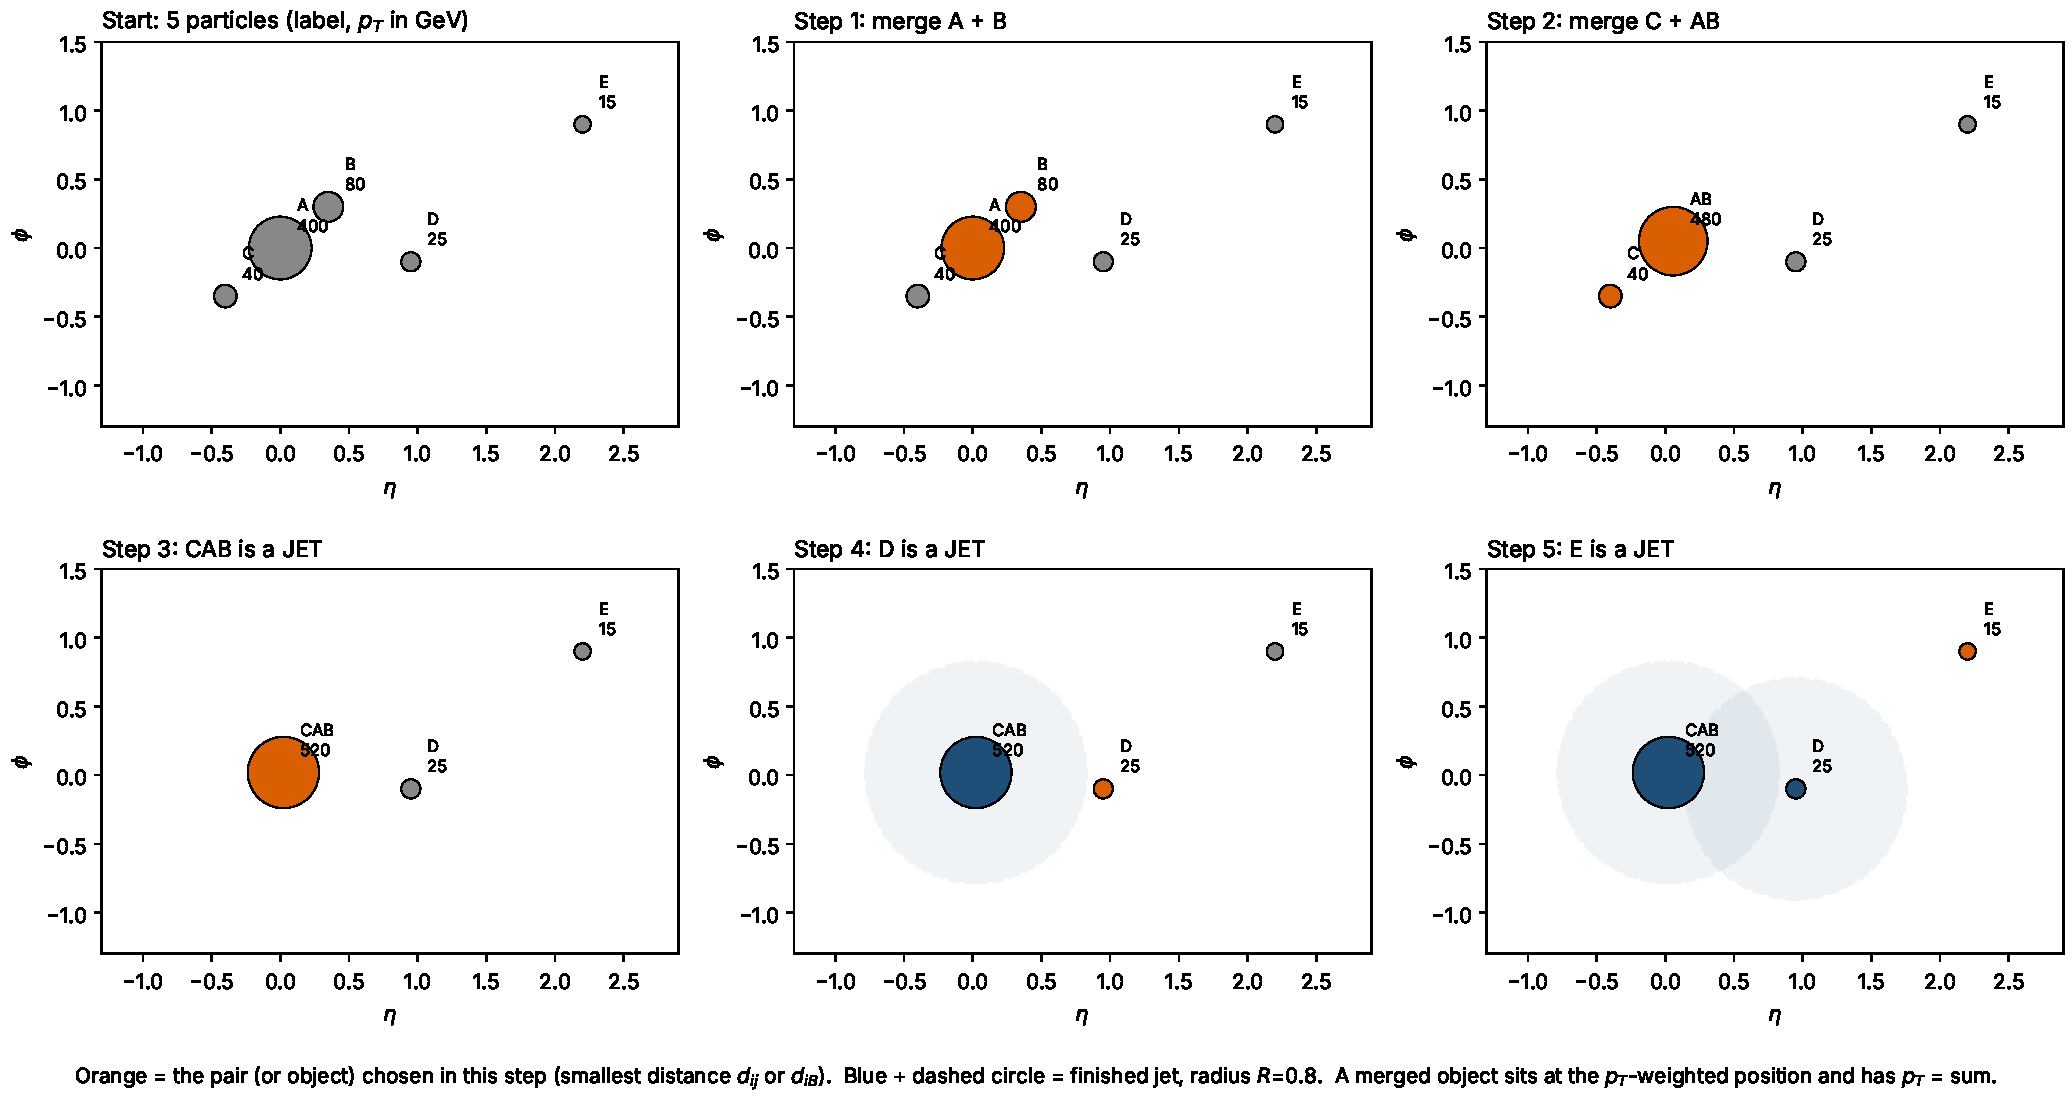
\includegraphics[width=\textwidth]{antikt2.pdf}
\caption{مراحل ساخته شدن جت‌ها با \lr{anti-$k_\mathrm{T}$}. رنگ نارنجی جفت یا شیئی است که در آن مرحله کوچک‌ترین فاصله ($d_{ij}$ یا $d_{iB}$) را دارد. رنگ آبی و دایره خط‌چین (شعاع $R=0.8$) جت تمام‌شده است. شیء ادغام‌شده در موقعیت وزن‌دار با $\pt$ قرار می‌گیرد و $\pt$ آن مجموع دو شیء است.}
\label{fig:antikt}
\end{figure}
ذره سخت \lr{A} ابتدا همسایه‌های خود \lr{B} و بعد \lr{C} را می‌بلعد و شیء \lr{CAB} با $\pt=400+80+40=520$~\lr{GeV} ساخته می‌شود. ذره‌های نرم هرگز اول با هم ادغام نمی‌شوند؛ جت دور هسته سخت رشد می‌کند و ذره‌های نزدیک‌تر زودتر جذب می‌شوند، برای همین جت شکلی گرد دارد. در مرحله بعد باید \lr{CAB} را با \lr{D} مقایسه کنیم که با $\Delta R=0.95$ از آن فاصله دارد. فاصله \lr{CAB} تا باریکه $d_{iB}=1/520^2\approx3.7\times10^{-6}$ است و فاصله تا \lr{D} برابر $d_{ij}=(0.95/0.8)^2/520^2\approx1.41\times3.7\times10^{-6}\approx5.2\times10^{-6}$ است. چون $d_{iB}<d_{ij}$، \lr{CAB} یک جت تمام‌شده می‌شود و \lr{D} به آن نمی‌پیوندد. \lr{D} و \lr{E} نیز با همین استدلال هر کدام یک جت نرم جدا می‌شوند.

جت‌های ساخته‌شده با این الگوریتم ذره مشترک ندارند، چون هر ذره دقیقاً به یک جت تعلق دارد؛ پس تعداد ذرات تشکیل‌دهنده و جرم جت‌های مختلف از هم مستقل‌اند. محور دو جت نیز همیشه بیش از $R$ از هم دور است، چون اگر دو شیء از $R$ نزدیک‌تر بودند ادغام می‌شدند؛ به همین دلیل نمودارهای $\Delta R$ بین دو جت از حدود \lr{0.8} شروع می‌شوند. از نظر هندسی، دایره‌های شعاع $R$ دو جت برای $R<\Delta R<2R$ هم‌پوشانی دارند (در شکل، \lr{CAB} و \lr{D} با $\Delta R=0.95$)، ولی ذره‌های ناحیه مشترک به جت سخت‌تر تعلق دارند و جت نرم‌تر در آن ناحیه بریده می‌شود. در نتیجه هیچ ذره‌ای بین جت منتخب و جت دیگری مشترک نیست و جت سخت یک مخروط تمیز است.

در این پروژه برای $\pt$ در خوشه‌بندی آستانه نگذاشتیم (\lr{inclusive\_jets(0)})، پس هر ذره نرمی که از ذره‌های سخت دورتر از $R$ بود خودش یک جت شد. به همین دلیل بدون آستانه، هر رویداد حدود ۳۳ تا ۳۵ جت دارد (شکل~\ref{fig:s1all}). این‌ها جت واقعی نیستند: جت واقعی آستانه می‌خواهد. تعداد جت‌های باقی‌مانده بعد از هر برش در شکل~\ref{fig:s1njets} (بخش~\ref{sec:cutflow}) آمده است. ما تنها جت‌های با \lr{$\pt>20$~GeV} را ذخیره می‌کنیم.
\widefig{s1_all_njets.pdf}{تعداد جت در هر رویداد بدون آستانه $\pt$.}{fig:s1all}

\section{ویژگی‌های ذرات تشکیل‌دهنده در داده}
\label{app:cons}
برای هر جتی که برش‌های تحلیل را بگذراند ($\pt>400$~\lr{GeV}، $|\eta|<2$ و دست‌کم ۳ ذره تشکیل‌دهنده)، ۱۷ ویژگی برای حداکثر ۱۰۰ ذره تشکیل‌دهنده ذخیره شده است. ذره‌ها به ترتیب $\pt$ مرتب می‌شوند و سخت‌ترین اول می‌آید؛ جت‌هایی که کمتر از ۱۰۰ ذره دارند با صفر پر می‌شوند. ورودی خوشه‌بندی سه چیز است: ردهای باردار با نوع ذره‌ای که \lr{Delphes} می‌دهد (علامت‌دار)، برجک‌های فوتونی که نوع ۲۲ می‌گیرند و برجک‌های هادرون خنثی که نوع ۱۳۰ می‌گیرند.

شش ویژگی اول تکانه و انرژی ذره در دستگاه آزمایشگاه‌اند: $p_x$، $p_y$، $p_z$، $E$، $E/E_\mathrm{jet}$ و $\pt$، و بعد از آن $p_T/p_{T,\mathrm{jet}}$. ویژگی‌های زاویه‌ای هشت‌تایی هستند: $\eta$، $\eta-\eta_\mathrm{jet}$، $\eta_\mathrm{rot}$، $\varphi$، $\varphi-\varphi_\mathrm{jet}$، $\varphi_\mathrm{rot}$ و فاصله $\Delta R=\sqrt{(\eta-\eta_\mathrm{jet})^2+(\varphi-\varphi_\mathrm{jet})^2}$ ذره تا محور جت، که در همه این‌ها اختلاف $\varphi$ به بازه $(-\pi,\pi]$ برگردانده می‌شود. دو ویژگی زاویه‌ای باقی‌مانده $\cos\theta=p_z/|\vec p|$ (زاویه قطبی نسبت به محور پرتو) و $\cos\theta_\mathrm{rel}=\vec p\cdot\vec p_\mathrm{jet}/(|\vec p|\,|\vec p_\mathrm{jet}|)$ (زاویه نسبت به محور جت) هستند. ویژگی هفدهم، نوع ذره $\mathrm{pdgId}$ است.

مختصات چرخیده را این‌طور می‌سازیم. اگر $(\eta_0,\varphi_0)$ موقعیت سخت‌ترین ذره و $(\eta_1,\varphi_1)$ موقعیت دومین ذره باشد، تعریف می‌کنیم $x_i=\eta_i-\eta_0$ و $y_i=\varphi_i-\varphi_0$ (با برگرداندن به $(-\pi,\pi]$). با زاویه
\begin{equation}
\alpha=\operatorname{atan2}(y_1,x_1),\qquad \vartheta=-\frac{\pi}{2}-\alpha
\end{equation}
مختصات چرخیده هر ذره چنین است:
\begin{equation}
\eta_{\mathrm{rot},i}=x_i\cos\vartheta-y_i\sin\vartheta,\qquad
\varphi_{\mathrm{rot},i}=x_i\sin\vartheta+y_i\cos\vartheta .
\end{equation}
برای دومین ذره، با $x_1=r\cos\alpha$ و $y_1=r\sin\alpha$ که $r$ فاصله آن تا سخت‌ترین ذره است، داریم $\eta_{\mathrm{rot},1}=r\cos(\alpha+\vartheta)=r\cos(-\pi/2)=0$ و $\varphi_{\mathrm{rot},1}=r\sin(\alpha+\vartheta)=r\sin(-\pi/2)=-r$. یعنی سخت‌ترین ذره در مبدأ و دومین ذره روی محور منفی $\varphi$ چرخیده قرار می‌گیرد؛ به همین دلیل $\eta_\mathrm{rot}$ دومین ذره همیشه صفر (در حد خطای عددی) و $\varphi_\mathrm{rot}$ آن همیشه نامثبت است و $\varphi_\mathrm{rot}$ سخت‌ترین ذره همیشه صفر است. این دو ویژگی ثابت اطلاعاتی ندارند و برای ذره‌های دیگر فقط شکل نسبی خوشه‌های ذره‌ها را نشان می‌دهند. نمودار همه این ویژگی‌ها در بخش~\ref{sec:particles} آمده است.

\end{document}
